\chapter{Научно-популярные статьи}

\section{Времена года}
\textit{Источник: \url{https://www.memorysecrets.ru/english-texts/vremena-goda-seasons.html}}

Каждое время года имеет свои плюсы и минусы. Давайте детальнее их разберем.

Весна (март, апрель, май) --- самое восхитительное время года. Несмотря на то, что весной \explainDetail{наблюдаются}{(по)наблюдаться}{to be observed} \explainDetail{ливни}{ливень}{shower (rain)}, многие люди \explain{воспринимают}{perceive} весну, как самое лучшее время года. Почему же так \explain{происходит}{happens}? \explain{Дело в том}{the thing is}, весна значит что-то новое для нас. Это шанс начать все заново, изменить жизнь к лучшему. Именно весной рожд\'{а}ется новая жизнь --- \explain{распускаются}{they bloom} почки и начинают цвести цветы.

Лето же (июнь, июль, август) --- это время отдыхать и просто получать удовольствие. Солнце светит с утра до ночи. Взрослые уходят в отпуск, дети --- на каникулы. Большинство людей проводят свои отпуска на море. Там можно не только \explainDetail{загореть}{загорать/загореть}{to tan}, но и встретить много незнакомых людей.

Осень (сентябрь, октябрь, ноябрь) можно разделить на две части --- начало осени и ее конец. В начале осени школьники снова возвращаются к учебе и садятся \explain{за парты}{behind the desks}. Лето постеп\'{е}нно переходит в осень. Но настроение ещё \explain{приподнятое}{elevated}. Вскоре желтые листья начнут осыпаться, и этот величественный пейзаж тоже не \explainDetail{позв\'{о}лит}{позвол\'{я}ть/позв\'{о}лить}{to allow} нам грустить. Втор\'{а}я часть осени не так очаров\'{а}тельна, как первая. Дожди, \explain{сл\'{я}коть}{mud} и грязь --- это то, что люди ненавидят больше всего.

Зима (декабрь, январь, февраль) \explain{на нос\'{у}}{фразеологизм: приближаться, близиться (обычно -- по времени)}, приближаются холода. Мы надеваем перчатки, шапки, шубы и вязаные шарфы. Иногда в эту пору школы закрывают на карантин с целью предотвратить распространение гриппа. Хорошая новость для учеников --- вторые зимние каникулы. Рождество тоже вот-вот наступит. На улице порошит снег, дети лепят снеговиков и играют в снежки. Скоро мы будем наряжать елку, вешать на нее различные шары и гирлянды. Пора встречать Новый год!

\section{Что такое изменение климата?}
\textit{Источник: \url{https://www.un.org/ru/climatechange/what-is-climate-change}}

Под изменением климата понимают \ed{долгосрочные}{долгоср\'{о}чный}{long-term (for a long period)} температурные изменения и изменение погодных \ed{условий}{усл\'{о}вие}{condition}. Хотя эти изменения м\'{о}гут быть естественными, как, например, \ed{циклические}{циклический}{cyclical} \ed{колебания}{колеб\'{а}ние}{fluctuation} солнечной активности, с \ed{1800-х}{1800-х}{тысячи восемьсотых} годов антропогенная деятельность является основным \explain{движущим фактором}{driving factor} изменения климата, \explain{главным образом}{mainly} за счёт \ed{сжигания}{сжигание}{burning; combustion} ископаемых видов топлива, таких как уголь, нефть и газ.

В результате сжигания ископаемых видов топлива образуются \explain{выбросы}{emissions} \ed{парниковых газов}{парник\'{о}вые г\'{а}зы}{greenhouse gases}, которые подобно одеялу \explain{окутывают}{they envelop} Землю, удерживая солнечное тело и \explain{повышая}{raising} температуру.

Примерами парниковых газов, выбросы которых вызывают изменение климата, являются \explain{дву\'{о}кись углер\'{о}да}{углекислый газ} и мет\'{а}н. Они образуются, например, при использовании бензина для езды на автомобилях или угля для отопления зданий. \explain{Расчистка земель и лесов}{the ``clearing'' of lang and forest} также может привести к \ed{высвобождению}{высвобожд\'{е}ние}{release} углекислого газа.
Главным источником выбросов метана являются \explain{м\'{у}сорные св\'{а}лки}{garbage dumps}.
К числу основных производителей выбросов относятся энергетика, промышленность, транспорт, здания, сельское хозяйство и землеп\'{о}льзование.

\begin{fancyquotes}
    Концентрация парниковых газов находится на самом высоком уровне за последние 2 миллиона лет
\end{fancyquotes}

И выбросы продолжают расти! В результате этого сейчас Земля на \explain{1,1°C}{одна целая, одна десятая градуса Цельсии} теплее, чем в конце 1800-х годов. Прошедшее десятилетие (2011–2020 г\'{о}ды) было самым тёплым в истории.

Хотя многие думают, что изменение климата означает в основном более высокие температуры, рост температуры -- это только начало истории. Поскольку Земля -- это система, где всё \explain{взаимосв\'{я}зано}{interconnected}, изменения в одной \explain{сфере}{here: area} могут повлиять на изменения во всех остальных.

В настоящее время к последствиям изменения климата относят, \explain{среди прочего}{among other things}, сильные \ed{з\'{а}сухи}{з\'{а}суха}{drought}, \explain{нехватку воды}{water shortage}, сильные пожары, повышение уровня моря, наводнения, \explain{т\'{а}яние}{melting (n.)} полярных льдов, катастрофические штормы и сокращение \ed{биоразнообр\'{а}зия}{биоразнообр\'{а}зие}{biodiversity}.

\begin{fancyquotes}
    Люди ст\'{а}лкиваются с различными последствиями изменения климата
\end{fancyquotes}

Изменение климата может \ed{сказ\'{а}ться}{ск\'{а}зываться/сказ\'{а}ться + на что}{affect} на нашем здоровье, способности \explain{выращивать}{to grow} \explain{продовольственные культуры}{food crops}, жильё, безопасности и работе.
Некоторые из нас уже сейчас более \ed{уязв\'{и}мы}{уязв\'{и}мый}{vulnerable} к \ed{воздействию}{возд\'{е}йствие}{impact (n)} изменения климата, например, люди, живущие в малых \ed{островн\'{ы}х}{островн\'{о}й}{insular} государствах и других развивающихся странах. Такие последствия, как повышение уровня моря и интрузия соленых вод, дост\'{и}гли такого уровня, что целые общ\'{и}ны были в\'{ы}нуждены \explain{пересел\'{и}ться}{to resettle}, а затяжные засухи \explain{подвергают}{subject; expose} людей риску г\'{о}лода. В будущем ожидается рост числа «климатических беженцев».

\begin{fancyquotes}
    Каждый дополнительный градус \ed{глобального потепления}{глобальное потепление}{global warming} \explain{имеет значение}{matters}
\end{fancyquotes}

В докладе Организации Объединённых Наций за 2018 год тысячи учёных и \ed{правительственных экспертов}{прав\'{и}тельственный эксп\'{е}рт}{gov't expert} согласились с тем, что \explain{ограничение}{limitation} роста глобальной температуры на уровне не более 1,5°C поможет нам избежать самых худших климатических последствий и \explain{сохранить}{save} кл\'{и}мат, \explain{приг\'{о}дный для жизни}{habitable}. Однако, согласно текущим национальным климатическим планам, ожидается, что глобальное потепление дост\'{и}гнет 2,7°C к концу столетия.

Хотя выбросы, вызывающие изменение климата, образуются во всех регионах мира и сказываются на всех, некоторые страны производят их в гораздо больших объёмах, чем другие. В то время как на 100 стран, которые производят меньше всего выбросов, приходится 3 процента от общего объема выбросов, \explain{доля}{share (n)} десяти стран, являющихся самыми крупными производителями выбросов, составляет 68 процентов. Хотя принятие мер по борьбе с изменением климата -- это дело всех и каждого, народы и страны, которые создают больше проблем, должны взять на себя большую ответственность и начать действовать первыми.

\begin{fancyquotes}
    Мы сталкиваемся с огромным \ed{вызовом}{вызов}{challenge}, но нам уже известны многие решения
\end{fancyquotes}

Многие решения в области изменения климата могут быть не только экономически выгодными, но и также улучшить нашу жизнь и защитить окружающую среду. У нас также есть глобальные структуры и соглашения, на основе которых осуществляются \ed{усилия}{усилие}{effort}, направленные на достижение прогресса, такие как цели в области \ed{устойчивого развития}{устойчивый развитие}{sustainable development}, Рамочная конвенция Организации Объединённых Наций об изменении климата и Парижское соглашение. Имеются три широкие категории действий: сокращение выбросов, адаптация к последствиям изменения климата и финансирование необходимых мер по адаптации.

\explain{Перевод}{Translation (meaning transition)} энергетических систем с ископаемого топлива на использование \ed{возобновляемых источников энергии}{возобновляемые источники энергии}{renewable energy sources}, таких как солнце или ветер, позв\'{о}лит сократить выбросы, вызывающие изменение климата. Но начинать нужно прямо сейчас. Несмотря на расширение коалиции стран, \explain{обязавшихся}{who pledged} достичь чистого нулевого уровня выбросов к 2050 году, около половины мер по сокращению выбросов должны быть осуществлен\'{ы} к 2030 году, с тем чтобы удержать потепление на уровне ниже 1,5°C. В период с 2020 по 2030 год производство ископаемого топлива должно сокращаться прим\'{е}рно на 6 процентов в год.

Цель адаптации к последствиям изменения климата состоит в том, чтобы защитить людей, их жилища, предприятия, источники средств к существованию, инфраструктуру и природные экосистемы. Эта деятельность касается не только нынешних последствий, но и тех, с которыми, вероятно, придётся столкнуться в будущем. Хотя меры по адаптации придётся принимать \explain{повсеместно}{everywhere}, в настоящее время приоритетное внимание необходимо уделять наиболее уязв\'{и}мым сло\'{я}м населения, у которых меньше всего ресурсов для того, чтобы \explain{противостоять}{resist} климатическим угр\'{о}зам. Это может \explain{окупиться}{pay off} \explain{сполна}{completely}. Например, системы раннего предупреждения \ed{стихийных бедствий}{стихийное бедствие}{natural disaster} спасают жизни и имущество и могут принести выгоды, в десятки раз превышающие первоначальные \explain{затраты}{costs}.

\begin{fancyquotes}
    Мы можем оплатить счет сейчас или дорого заплатить в будущем
\end{fancyquotes}

Меры по борьбе с изменением климата требуют значительных финансовых \ed{вложений}{вложение}{investment} со стороны правительств и делов\'{ы}х кругов. Однако \explain{бездействие}{inaction} в отношении климата обходится гораздо дороже. Одним из важнейших шагов является выполнение \ed{промышленно развитыми странами}{промышленно развитая стран\'{а}}{industrialised countries} своих обязательств по предоставлению 100 миллиардов долларов в год \ed{развивающимся странам}{развив\'{а}ющаяся стран\'{а}}{developing country}, с тем чтобы они могли адаптироваться и перейти к более «зеленой» экономике.


\newpage
\section{Причины изменения климата}
\textit{Источник: \url{https://www.un.org/ru/science/causes-effects-climate-change}}



\textbf{Производство электроэнергии}

Значительная доля глобальных выбросов связана с производством электроэнергии и тепла путем сжигания ископаемых видов топлива. Бóльшая часть электроэнергии по-прежнему производится посредством сжигания угля, нефти или газа, в результате чего образуются углекислый газ и закись азота – мощные парниковые газы, которые покрывают Землю и \explain{задерживают}{trap; hold} солнечное тепло. Во всем мире чуть более четверти электроэнергии вырабатывается \explain{за счёт}{here it means ``by means of,'' but it can also mean ``at the expense of.''} ветра и солнца и поступает из других возобновляемых источников, которые, в отличие от ископаемых видов топлива, практически не \explain{выделяют}{emit} в атмосферу парниковых газов или \ed{загрязняющих веществ}{загрязняющее вещество}{pollutant}.

\textbf{Изготовление\footnote{изготовление: manufacturing} товаров}

Предприятия обрабатывающей и других отраслей промышленности производят выбросы, в большинстве случаев являющиеся результатом сжигания ископаемых видов топлива в целях выработки энергии, необходимой для получения цемента, железа, стали, электронных устройств, \ed{пластмасс}{пластм\'{а}сса}{plastic}, одежды и других товаров.
При добыче полезных ископаемых и других промышленных процессах, \explain{равно как}{as well as} и при строительстве, также выделяются газы. Машины, используемые в производственном процессе, \explain{зачаст\'{у}ю}{often} работают на угл\'{е}, нефти или газе, а некоторые материалы, такие как пластмассы, производятся из химических веществ, получаемых из ископаемых видов топлива. Обрабатывающая промышленность является одним из крупнейших источников выбросов парниковых газов в мире.

\textbf{Вырубка лесов\footnote{в\'{ы}рубка лес\'{о}в: deforestation}}

В результате вырубки лесов для создания ферм или пастбищ либо по иным причинам образуются выбросы, поскольку вырубаемые деревья высвобождают накопленный углерод. Ежегодно уничтожается около 12 млн гектаров леса. Поскольку леса \explain{поглощают}{absorb} углекислый газ, их уничтожение также ограничивает способность природы удерживать выбросы в атмосферу. \ed{Обезл\'{е}сение}{обезл\'{е}сение}{deforestation} \explain{наряду с}{along with; alongside} сельским хозяйством и другими изменениями в землепользовании является причиной примерно четверти глобальных выбросов парниковых газов.

\textbf{Использование транспорта}

Большинство автомобилей, грузовиков, кораблей и самолётов работают на ископаемых видах топлива. Это делает транспорт одним из главных источников выбросов парниковых газов, особенно выбросов углекислого газа. Наибольшая их часть приходится на дорожные транспортные средства в связи со сжиганием продуктов нефтепереработки, таких как бензин, в двигателях внутреннего сгорания. При этом выбросы морск\'{и}х и воздушных суд\'{о}в продолжают расти. На транспорт приходится почти четверть глобальных выбросов углекислого газа, связанных с энергоснабжением. \explain{Существующие тенденции}{Existing trends} \explain{указывают на}{indicate} вероятность значительного увеличения энергопотребления в транспортном секторе в ближайшие годы.

\textbf{Производство продуктов питания}

Производство продуктов питания прив\'{о}дит к выбросам углекислого газа, метана и других парниковых газов разными путями, включая вырубку лесов и расчистку земель для ведения сельского хозяйства и выпаса скота, работу пищеварительных систем коров и овец, производство и применение удобрений и навоза для выращивания сельскохозяйственных культур и использование энергии для эксплуатации сельскохозяйственного оборудования или рыболовецких судов, обычно работающих на ископаемых видах топлива. Все это делает производство продуктов питания одним из основных факторов, способствующих изменению климата. Выбросы парниковых газов также связаны с \ed{упаковкой}{упаковка}{packaging} и \ed{распростран\'{е}нием}{распростран\'{е}ние}{here: distribution} продуктов питания.

\textbf{Энергоснабжение зданий\footnote{энергоснабжение зданий: energy supply of buildings}}

В мировом масштабе жил\'{ы}е и коммерческие здания потребляют более половины всей электроэнергии. В связи с продолжающимся использованием угля, нефти и природного газа для целей отопления и \ed{охлаждения}{охлаждение}{cooling} они выбрасывают значительные количества парниковых газов. В последние годы повышение \ed{спроса}{спрос}{demand} на энергию для \ed{отопления и охлаждения}{отопление и охлаждение}{heating and cooling} с р\'{о}стом ч\'{и}сленности влад\'{е}льцев \ed{кондиционеров}{кондицион\'{е}р}{air conditioner} и увеличение потребления электричества для \ed{освещения}{освещение}{lighting} и обеспечения работы бытовой техники и подключенных устройств способствовали увеличению выбросов углекислого газа, производимых зданиями и связанных с энергоснабжением.

\textbf{Слишком интенсивное потребление}

Ваш дом и использование электроэнергии, то, как вы передвигаетесь, то, что вы едите, и количество того, что вы выбрасываете, влияют на выбросы парниковых газов. Это же можно сказать о потреблении таких товаров, как одежда, электронные устройства и пластмассы. Значительная часть глобальных выбросов парниковых газов связана с частными домохозяйствами. Наш образ жизни оказывает глубокое воздействие на нашу планету. Самые \explain{состоятельные}{состоятельный}{wealthy; well-off} л\'{и}ца несут наибольшую ответственность\footnote{Recall: нести ответственность: to have responsibility}: на 1 процент самых богатых жителей планеты в совокупности приходится больше выбросов парниковых газов, чем на 50 процентов беднейшего населения.

На основе различных источников ООН

\newpage
\section{Последствия изменения климата}
\textit{Источник: \url{https://www.un.org/ru/science/causes-effects-climate-change}}


\textbf{Повышение температур}

С увеличением концентрации парниковых газов растёт и глобальная температура земной поверхности. Последнее десятилетие --- 2011–2020 годы --- стало самым тёплым за всю историю наблюдений. С 1980-х годов каждое десятилетие было теплее предыдущего. Почти во всех районах суши наблюдается увеличение количества жарких дней и периодов аномальной жары. Повышение температуры увеличивает количество заболеваний, связанных с жарой, и затрудняет работу на открытом воздухе. Природные пожары легче возникают и быстрее распространяются в более жарких условиях. Температура в Арктике повышалась по крайней мере вдвое быстрее, чем в среднем по миру.

\textbf{Усиление штормов}

Многие регионы \ed{столкн\'{у}лись}{ст\'{а}лкиваться/столкн\'{у}ться + с}{were faced with} с увеличением интенсивности и частоты \ed{разрушительных}{разрушительный}{destructive} штормов. При повышении температуры \explain{испаряется}{evaporates} больше \ed{влаги}{влага}{humidity}, что усиливает ливневые дожди и наводнения, вызывая более опасные штормы. На частоту и масштабы тропических штормов также влияет потепление океана. Циклоны, ураганы и тайфуны формируются в тёплых водах у поверхности океана. Такие ураганы нередко разрушают дом\'{а} и \explain{населенные пункты}{populated areas; settlements}, становясь причиной гибели людей и огромных экономических потерь.

\textbf{Усиление з\'{а}сухи}

Изменение климата меняет степень доступности воды, делая её более дефицитным ресурсом в растущем числе регионов. Глобальное потепление усугубляет нехватку воды в регионах, и без того испытывающих её дефицит, и увеличивает риск сельскохозяйственных засух, влияющих на урожай, и экологических засух, повышающих уязвимость экосистем. Засухи также могут вызывать разрушительные \explain{песчаные}{sandy} и пыльные бури, способные перемещать миллиарды тонн песка через континенты. Пустыни расширяются, сокращая площадь земель для выращивания продовольственных культур. Сегодня многие люди постоянно сталкиваются с угр\'{о}зой нехватки воды.

\textbf{Потепление и повышение уровня океана}

Океан \explain{поглощает}{absorbs} бóлчьшую часть тепла, образующегося в процессе глобального потепления. За последние двадцать лет скорость, с которой океан \explain{нагревается}{heats up}, сильно возросла на всех его глубинах. По мере потепления океана его объём увеличивается, поскольку при нагревании вода расширяется. Таяние ледовых щитов также приводит к повышению уровня моря, \explain{угрожая}{threatening} прибрежным и островным сообществам. Кроме того, океан поглощает из атмосферы углекислый газ. При этом увеличение количества углекислого газа повышает кислотность океана, что ставит под угрозу морскую флору и ф\'{а}уну и коралловые рифы.

\textbf{Исчезновение видов}

Изменение климата создает риски для выживания видов на суше и в океане. Эти риски возрастают по мере повышения температуры. Мир, положение в котором усугубляется изменением климата, теряет виды в тысячу раз быстрее, чем когда-либо в письменной истории человечества. Миллион видов находится под угрозой исчезновения в течение следующих нескольких десятилетий. В число многочисленных угроз, связанных с изменением климата, входят лесные пожары, экстремальные погодные условия и инвазивные вредители и заболевания. Некоторые виды смогут сменить место обитания и выжить, а другие нет.

\textbf{Нехватка продуктов питания}

В группу причин глобального роста распространенности голода и неполноценного питания входят климатические изменения и увеличение количества экстремальных погодных явлений. Рыбные ресурсы, сельскохозяйственные культуры и домашний скот могут быть уничтожены или стать менее продуктивными. В связи с закислением океана морские ресурсы, обеспечивающие питание для миллиардов людей, находятся под угрозой. Изменения снежного и ледяного покрова во многих арктических регионах нарушили систему снабжения продовольствием, обеспечиваемым за счет пастбищного животноводства, охоты и рыболовства. Тепловой стресс может уменьшать количество воды и пастбищ, что приводит к снижению урожайности сельскохозяйственных культур и негативным образом сказывается на поголовье скота.

\textbf{Увеличение рисков для здоровья}

Изменение климата – это самая большая угроза для здоровья людей. Его последствия уже наносят вред здоровью в связи с загрязнением воздуха, распространением заболеваний, возникновением экстремальных погодных явлений, вынужденным перемещением, оказанием давления на психику и обострением проблем голода и неполноценного питания в местах, где люди не могут выращивать продовольственные культуры или обеспечить наличие достаточного количества пищевых продуктов. Экологические факторы ежегодно уносят жизни около 13 млн человек. Изменение погодных условий приводит к распространению заболеваний, а экстремальные погодные явления увеличивают смертность и затрудняют работу систем здравоохранения.

\textbf{Нищета и вынужденное перемещение}

Изменение климата усиливает факторы, ввергающие людей в нищету и не позволяющие им исправить ситуацию, в которой они оказались. Наводнения могут смести городские трущобы, разрушив дома и уничтожив источники средств к существованию. Жара может затруднить работу на открытом воздухе. Нехватка воды может повлиять на урожай. В последние десять лет (2010–2019 годы) связанные с погодой явления приводили к вынужденному перемещению в среднем около 23,1 млн человек в год, повышая риск оказаться в нищете для еще большего числа людей. Большинство беженцев прибывают из самых уязвимых стран, наименее готовых адаптироваться к последствиям изменения климата.

\textit{На основе различных источников ООН}

\newpage
\section{Человечество ждёт серия масштабных природных катастроф}

\textit{В чем причина стихийных бедствий ближайшего будущего?}

\textit{Источник: \url{https://lenta.ru/articles/2022/10/17/trilliondollarbaby/}}

В скором будущем человечество ожидает уникальное для этого столетия явление. Так называемая Ла-Нинья — феномен, с которым связано широкомасштабное охлаждение вод Тихого океана, — грозит оказаться тройной. Последствия Ла-Ниньи, чье название с испанского можно перевести как «девочка», могут стать катастрофическими. Если прогноз сбудется, хаос природных катаклизмов на планете только усилится. В таком сценарии глобальный ущерб от стихийных бедствий достигнет триллиона долларов. Роковая «малышка» — в материале «Ленты.ру».

\textbf{Горячо-холодно.} Нынешняя затяжная Ла-Нинья началась в сентябре 2020 года. Явление уже успело усугубить засуху и наводнения в различных частях мира, а теперь же Всемирная метеорологическая организация (ВМО) предупредила, что явление затянется надолго. С вероятностью в 70 процентов оно сохранится до ноября, с вероятностью в 55 процентов — до февраля следующего года.

Ситуация, как подчеркнул генеральный секретарь ВМО Петтери Таалас, складывается исключительная. В нынешнем столетии природный феномен может охватить сразу три зимы в Северном полушарии и три лета в Южном. Если прогноз ВМО окажется верным, то тройная Ла-Нинья станет третьей по счету за всю историю наблюдений — с 1950 года подобное случалось лишь дважды.

Ла-Нинья (исп. La Niña — малышка, девочка) — это снижение температуры поверхностных вод в центральной и восточной частях Тихого океана. На этом фоне усиливаются стабильные восточные ветра, которые гонят теплую воду от берегов Перу и Чили в сторону Индонезии и Австралии. В результате средние температуры воздуха во всем мире понижаются.

Явление с противоположным эффектом, когда температура воды и воздуха у побережья Южной Америки растет, называют Эль-Ниньо (исп. El Niño — малыш, мальчик), а его чередование с Ла-Ниньей — Южной осцилляцией. Феномен описал британский ученый Гилберт Уокер в 1923 году, однако впервые на него обратили внимание перуанские рыбаки в 1600 годах — Ла-Нинья для них не имела критического значения, но потепление воды при Эль-Ниньо плохо сказывалось на уловах.

На климат нашей планеты Ла-Нинья оказывает охлаждающий эффект, который достигает своего максимума на второй год после ее пика. Характерными проявлениями феномена метеорологи называют прохладную и влажную зиму на севере Европы и в Великобритании, дождливое лето в Индонезии и Австралии, сильные муссоны (ветры, дующие с суши на океан) в Юго-Восточной Азии, холода в Южной части Африки. В этот период зима на Дальнем Востоке в России, в Японии, Корее, Канаде, на севере США обычно бывает более снежной и ветреной. В Техасе, Флориде и других южных штатах Америки, наоборот, случаются сильные засухи.

При этом связанное с деятельностью человека изменение климата, как отмечают ученые, усиливает воздействие Южной осцилляции на окружающую среду. ВМО выяснила, что за последние 50 лет число стихийных бедствий пятикратно увеличилось.

\begin{fancyquotes}
    Это означает более длительные и интенсивные волны тепла, более длительные засухи, более масштабные лесные пожары и более разрушительные наводнения. Усиленный изменением климата эффект от Ла-Ниньи носит глобальный характер

    \begin{flushright}
        Билл Пацертамериканский \\
        океанограф и климатолог
    \end{flushright}
\end{fancyquotes}

По словам ученой из Национального управления океанических и атмосферных исследований при министерстве торговли США Антониетты Капотонди, сила воздействия Южной осцилляции на климат непредсказуема — не наблюдалось двух абсолютно одинаковых по эффекту Эль-Ниньо и Ла-Ниньи. «Мы видели, насколько разнообразными могут быть последствия Южной осцилляции. Эта вариативность усложняет прогнозы по влиянию изменения климата на будущие Эль-Ниньо и Ла-Нинья», — пояснила исследовательница.

Ученые предполагают, что явления Эль-Ниньо и Ла-Нинья в перспективе будут случаться чаще. На фоне активного загрязнения планеты выбросами парниковых газов к концу XXI века они будут возникать не один раз в 20 лет, а раз в десятилетие. При этом осадки сместятся на восток вдоль экваториальной части Тихого океана во время Эль-Ниньо и на запад во время последствий Ла-Ниньи.

При увеличении периодичности и амплитуды Южной осцилляции экстремальные погодные явления будут более выраженными. Некоторые эффекты воздействия глобального потепления на протекание Эль-Ниньо и Ла-Ниньи уже стали очевидными — к примеру, тихоокеанские штормы заметно участились и усилились. В 2020 году зафиксировали рекордные 30 таких ураганов, в 2021-м — 21, а в 2022 — 14.

\textbf{Всем досталось.} Связанные с Ла-Ниньей экстремальные погодные условия затронули многие регионы планеты. Так, засуха накрыла западные части США и Канады, практически опустошив находящиеся на этих территориях водоемы. В результате возник дефицит пресной воды — ее не хватает ни для поливов сельскохозяйственных земель, ни для производства энергии на гидроэлектростанциях. В частности, в Техасе засуха привела к огромным потерям урожая хлопка — цены на него достигли десятилетнего максимума в начале 2022 года. По словам главного исполнительного директора компании Plains Cotton Growers Inc Коди Бессета, долговременная жара вкупе с практическим отсутствием осадков рискуют сделать 2022 год самым сложным для производства сельскохозяйственных культур. Эксперт прогнозирует, что производители недосчитаются более половины привычного объема урожая.

Продолжительная сухая погода также нанесла ущерб урожаю кофе, сахара и апельсинов в Бразилии, которая считается крупнейшим в мире экспортером этих трех культур. Помимо этого, экстремальные погодные условия нарушили работу предприятий по добыче железной руды в стране — в том числе второго по величине в мире производителя Vale SA.

В Аргентине засуха сказалась на посевах сои и кукурузы, которые играют ключевую роль в торговом балансе страны, переживающей острый экономический кризис. Многолетняя нехватка осадков также высушила ключевой водный путь — реку Парану. Поэтому фермеры и продавцы сельхозтоваров столкнулись с дополнительными расходами на логистику — им приходится платить внушительные суммы за отправку товаров через альтернативные порты.

На Австралию, наоборот, обрушились проливные дожди. Ливнями затопило большую часть штатов Новый Уэльс, Квинсленд и Виктория. Наводнения привели к гибели более 20 человек и разрушили более 15 тысяч домов. Страховые выплаты при этом превысили три миллиарда долларов.

Сильные дожди негативно сказались на качестве урожая уже выросших зерновых культур, а также задержали время посева ячменя и пшеницы. Кроме того, от разлива водоемов под угрозой выхода из строя оказались металлургические шахты в Новом Южном Уэльсе и Квинсленде — они являются крупнейшими в мире экспортерами сырья для производства стали. Другим катастрофическим последствием стала гибель животных. Так, связанные с Ла-Ниньей теплые течения в сторону востока погубили пингвинов, которых массово выбросило на пляжи Новой Зеландии.

Пакистан вызванные Ла-Ниньей обильные ливни поставили под угрозу дефолта. Страна подверглась беспрецедентным наводнениям, в результате которых были разрушены десятки миллионов домов, погибло почти 1500 человек. Кроме того, чрезмерные осадки повредили более 70 процентов посевов риса в провинции Синд. Нанесенный стихийными бедствиями ущерб аналитики оценивают в 30 миллиардов долларов. Южноазиатская страна и так страдает от сокращения валютных резервов и самой высокой инфляции за последние десятилетия, а природные факторы лишь усугубят тяжелое экономическое положение.

По данным Международной федерации обществ Красного Креста и Красного Полумесяца, разрушительные наводнения случились также в Бангладеш и Индии — от них пострадали более 7,2 миллиона человек и оказались поврежденными более 300 тысяч домов.

\textbf{Час расплаты.} Эксперты убеждены, что связанные с Ла-Ниньей погодные циклы усугубляют уже существующие глобальные проблемы. «Когда добавляются экстремальные погодные условия, это просто создает сценарий для более высоких цен на энергию, более высоких цен на продукты питания и большей инфляции. Это негативно для мировой экономики», — пояснил президент и основатель Pento Portfolio Strategies Майкл Пенто.

Ущерб от вызванных Ла-Ниньей засух, штормов и наводнений аналитики оценивают в десятки миллиардов долларов. Однако в этот раз природные катаклизмы случались так часто в разных уголках планеты, что реальную сумму потерь сложно вычислить. Получить представление о размере ущерба можно на основании данных страховых компаний. Как сообщают в аналитической и консалтинговой фирме Aon, в 2020 году стихийные бедствия обошлись миру в 268 миллиардов долларов, а в 2021-м — в дополнительные 329 миллиардов долларов.

\begin{framed}
    \begin{center}
        {\Huge
            1 триллион долларов
        }

        {\Large
            составит глобальный ущерб от последствий Ла-Ниньи
        }
    \end{center}
\end{framed}

Если будущий масштаб стихийных бедствий окажется соизмеримым с прошлыми годами, то к концу 2023-го сумма ущерба от Ла-Ниньи может достичь или даже превысить один триллион долларов. При этом речь идет не только о повреждении имущества и потерях урожая. От погодных условий зависят цены на разные товары по всему миру — от чашки кофе до угля, который используют для производства стали. Помимо войн, Ла-Нинья — единственное событие, оказывающее влияние на глобальные рынки и почти все отрасли экономики, считают эксперты.

\textbf{Выход есть?} Сократить риск негативных для планеты последствий явления можно за счет снижения антропогенного воздействия на климат — сокращения уровня эмиссии парниковых газов. Для этого, прежде всего, необходимо отказаться от использования ископаемого топлива — угля, нефти, природного газа и прочих горючих минералов — в пользу возобновляемых источников энергии, таких как солнечный свет, ветер и вода.

На протяжении нескольких десятилетий лидирующие позиции по энергопереходу занимает Евросоюз (ЕС) — в странах блока заметная доля в энергобалансе приходится на зеленые источники. Власти ЕС также поставили амбициозные цели по спасению планеты. Согласно опубликованной в 2021 году стратегии по борьбе с изменением климата, к 2030 году выбросы парниковых газов на территории Европы должны сократиться на 55 процентов относительно уровня 1990 года, а к 2050-му — быть полностью компенсированы.

Однако специальная военная операция России, начатая в феврале на Украине, вынудила ЕС поступиться важной целью. Блок стран резко сократил импорт дешевого российского газа (с 40 процентов в 2021 году до 7 процентов от общего объема) и столкнулся с энергетическим кризисом, так как существующих солнечных, ветряных и гидроэлектростанций недостаточно для обеспечения бесперебойной подачи тепла и света. Чтобы компенсировать нехватку, Европе пришлось вернуться к использованию сильно вредящих планете угля и мазута.

Все это делает недостижимыми цели Парижского соглашения по климату, которое подразумевает сдерживание роста среднемировых температур на отметке 1,5 градуса Цельсия относительно доиндустриального уровня. По прогнозам ученых, даже без учета наихудших сценариев средняя температура на планете повысится от 2,1 до 3,9 градуса Цельсия к 2100 году.

Межправительственная группа экспертов по изменению климата ООН уже предрекла человечеству неминуемую глобальную катастрофу. По прогнозам ученых, повышение температуры на планете в ближайшие десятилетия достигнет критических значений для сельского хозяйства и здравоохранения, а эффект глобального потепления ощутят на себе все страны мира.

Поскольку рост среднемировых температур продолжается, а глобальные выбросы СО2 не сокращаются, вероятно, Эль-Ниньо и Ла-Нинья станут лишь усиливаться, а вместе с ними увеличится и число катастрофических явлений. Среди угроз — более интенсивные дожди, наводнения, сильнейшая засуха во многих регионах, лесные пожары, опасность для прибрежных территорий из-за подъема уровня Мирового океана, усиление таяния вечной мерзлоты. Все это способно привести к затяжным экономическим кризисам, массовым проблемам со здоровьем и гибели людей и животных.

\newpage
\section{Городск\'{а}я жизнь}
Вы никогда не думали о последствиях жизни в городе? Казалось бы, \explain{на первый взгляд}{at first sight}, что жизнь в больших экономических и культурных центрах имеет только преимущества, но дальнейшее рассмотр\'{е}ние показывает, что она имеет и \explain{недостатки}{недостаток: disadvantage}.

С \explain{положительной}{полож\'{и}тельный/-ая: positive} стороны, легче найти работу в городе, потому что там обычно много ресторанов, кафе, гостиниц, школ, библиотек, музеев и т.д. Кроме того, жители города имеют прекрасную возможность посетить множество культурных и развлекательных учреждений, таких как музеи, галереи, ночные клубы, дискотеки и многое другое.

С другой стороны, жителям города \explain{приходится}{приходиться/прийтись: have to} жить в загрязненной атмосфере из-за интенсивного автомобильного движения и \explain{промышленных}{industrial} \explain{предприятий}{предпри\'{я}тие: enterprise}. Это может \explain{вызвать}{to cause} \explain{заболевания}{disease} лёгких и проблемы с сердцем. Кроме того, городской образ жизни довольно \explain{напряженный}{intense}, \explain{поскольку}{since/because} приходится много работать, много ездить на автомобиле и, в результате, стоять в пробках...

В заключение, городская жизнь имеет некоторые преимущества. Тем не менее, она также \explain{может нанести ощутимый вред}{can cause significant damage}, так что местные власти должны сделать несколько важных решений, например, они должны \explain{запретить}{[запрещать] to ban} промышленные предприятия в городах и вблизи городов, которые загрязняют воздух и воду токсичными парами.

\newpage
\section[Загрязнение окружающей среды]{Причины и последствия загрязнения окружающей среды}
\textit{Источник: \url{https://bit.ly/3NV3JeZ}}

Загрязнение окружающей среды в настоящее время является самой большой проблемой, с которой сегодня \explain{ст\'{а}лкивается}{faces, is facing} мир. Наприм\'{е}р, в Соединенных Штатах 40\% рек и 46\% озёр слишком загрязнен\'{ы} для \ed{рыбной л\'{о}вли}{рыбная ловля}{fishing}, \ed{купания}{купание}{bathing} и водных организмов. Это \explain{неудивительно}{not surprising}, когда ежегодно в американские воды \explain{сбрасывается}{dumped} 1,2 триллиона галлонов \explain{неочищенных}{untreated} ливневых вод, промышленных \ed{отходов}{отх\'{о}ды}{waste} и неочищенных \ed{сточных вод}{ст\'{о}чные в\'{о}ды}{sewage}.

Одна треть верхнего \ed{слоя}{спой}{layer} \ed{почвы}{почва}{soil} в мире уже деградирована, и \explain{с учётом}{taking into account} нынешних темпов деградации почвы, вызванной неправильными методами ведения сельского хозяйства и промышленности, а также \ed{обезлесением}{обезлесение}{deforestation}, большая часть верхнего слоя почвы в мире может исчезнуть в течение следующих 60 лет.

Великий смог 1952 года унёс жизни 8000 человек в Лондоне. Это событие \explain{было вызвано}{was caused (by)} периодом холодной погоды \explain{в сочетании с}{in conjunction with} безветренными условиями, которые сформировали \explain{плотный}{dense} слой переносимых по воздуху загрязнителей, в основном от угольных электростанций, над городом.

Существует множество источников загрязнения, каждый из которых по-своему влияет на окружающую среду и живые организмы. В этой статье обсуждаются проблема загрязнения и последствия различных видов загрязнения.

\textbf{Причины.} Причины загрязнения не \explain{ограничиваются}{are limited} только выбросами \ed{ископаемого топлива}{ископ\'{а}емое т\'{о}пливо}{fossil fuel} и \ed{углерода}{углерод}{carbon}. Существует множество других типов загрязнения, включая химическое загрязнение \ed{водоёмов}{водоём}{reservoir} и п\'{о}чвы в результате неправильной утилизации и сельскохозяйственной деятельности, а также шумов\'{о}е и светов\'{о}е загрязнение, создаваемое городами и урбанизацией в результате роста населения.

\textbf{Загрязнение воздуха.}
Существует два типа \ed{загрязнителей}{загрязн\'{и}тель}{pollutant} воздуха: \ed{первичные}{перв\'{и}чный}{primary} и \ed{вторичные}{вторичный}{secondary}. Первичные загрязнители выбрасываются \explain{непосредственно}{directly} из их источника, в то время как вторичные загрязнители образуются, когда первичные загрязнители вступают в реакцию в атмосфере.

\ed{Сжигание}{сжиг\'{а}ние}{burning, combustion} ископаемого топлива для тр\'{а}нспорта и электричества производит как первичные, так и вторичные загрязнители и является одним из крупнейших источников загрязнения воздуха.

\ed{Выхлопные газы}{выхлопные газы}{traffic fumes; exhaust fumes} автомобилей содержат опасные газы и \explain{твёрдые частицы}{solid particles}, включая \ed{углеводороды}{углеводород}{hydrocarbon}, оксиды азота и монооксид углерода. Эти газы \explain{поднимаются}{rise} в атмосферу и \explain{вступают в реакцию}{react} с другими атмосферными газами, создавая ещё б\'{о}лее токсичные газы.

По данным Института Земли, интенсивное использование \ed{удобрений}{удобрение}{fertiliser} в с\'{е}льском хоз\'{я}йстве является основным источником загрязнения воздуха \ed{мелкими частицами}{мелкие частицы}{microparticles}, что \explain{затронуло}{affected} большую часть Европы, России, Китая и США. Считается, что уровень загрязнения, вызванного сельскохозяйственной деятельностью, \explain{превышает}{exceeds} все другие источники загрязнения воздуха мелкими частицами в этих странах.

\ed{Аммиак}{амми\'{а}к}{ammonia} -- это основной загрязнитель воздуха, \explain{образующийся}{emerging} в результате сельскохозяйственной деятельности. Аммиак попадает в воздух в виде газа из концентрированных отходов животноводства и полей, которые \explain{чрезм\'{е}рно}{excessively} уд\'{о}брены.

Затем этот \explain{газообразный}{gaseous} аммиак соединяется с другими загрязнителями, такими как оксиды и сульфаты азота, образующиеся в транспортных средствах и промышленных процессах, с образованием аэрозолей. Аэрозоли -- это \explain{крошечные}{tiny} частицы, которые могут \explain{проникать}{permeate} глубоко в лёгкие и вызывать сердечные и лёгочные заболевания.

Другие сельскохозяйственные загрязнители воздуха включают пестициды, \explain{гербициды}{herbicides} и фунгициды. Все это также способствует загрязнению воды.

\textbf{Загрязнение воды.}
Загрязнение \ed{питательными веществами}{пит\'{а}тельные веществ\'{а}}{nutrients} вызывается сточными водами и удобрениями. Выс\'{о}кие уровни питательных веществ в этих источниках попадают в водоемы и способствуют росту \ed{водорослей}{водоросли}{algae} и \ed{сорняков}{сорняк}{weed}, что может сделать воду \ed{непригодной}{непригодный}{unusable; unfit} для \ed{питья}{питьё}{drinking} и \explain{истощить}{deplete} кислород, что \explain{приведет к гибели}{will lead to death} водных организмов.

Пестициды и гербициды, \explain{применяемые}{used; applied} для сельскохозяйственных культур и жил\'{ы}х районов, концентрируются в почве и перен\'{о}сятся в грунтовые воды с дождевой водой и стоками. По этим причинам каждый раз, когда кто-то пробуривает \ed{скважину}{скважина}{well (water well)} на воду, её необходимо проверять на \explain{наличие}{availability} загрязняющих веществ.

Промышленные отходы являются одной из основных причин загрязнения воды, поскольку они создают первичные и вторичные загрязнители, включая \ed{серу}{сера}{sulfur}, \explain{свинец}{lead} и \explain{ртуть}{mercury}, нитраты и фосфаты, а также разливы нефти.

В \ed{развивающихся странах}{развив\'{а}ющиеся стр\'{а}ны}{developing countries} около 70\% \explain{твёрдых отходов}{solid waste} сбрасывается непосредственно в океан или море. Это вызывает серьёзные проблемы, включая причинение вреда и убийство \ed{морских существ}{морские существа}{sea creatures}, что \explain{в конечном итоге}{eventually} влияет на людей.

\textbf{Загрязнение земли и п\'{о}чвы.}
Загрязнение земель -- это разрушение зем\'{е}ль в результате деятельности человека и неправильного использования земельных ресурсов. Это происходит, когда люди наносят на почву химические вещества, такие как пестициды и гербициды, неправильно утилизируют отходы и \explain{безответственно}{irresponsibly} \explain{эксплуатируют}{exploit} полезные ископаемые при \ed{добыче}{добыча}{mining} полезных ископаемых.

Почва также загрязняется из-за протекающих подземных септиков, канализационных систем, вымывания вредных веществ со \ed{свалок}{свалка}{landfill} и прям\'{о}го сбр\'{о}са сточных вод промышленными \ed{предприятиями}{предприятие}{enterprise} в реки и океаны.

Дождь и наводнение могут переносить загрязнители с других уже загрязнённых зем\'{е}ль в п\'{о}чву в других местах.

Избыточное \explain{земледелие}{agriculture} и чрезм\'{е}рный \explain{в\'{ы}пас}{grazing} в результате сельскохозяйственной деятельности прив\'{о}дят к тому, что п\'{о}чва теряет свою питательную ценность и структуру, вызывая деградацию почвы, ещё один тип загрязнения почвы.

Свалки могут вымывать вредные вещества в почву и водные пути и создавать очень неприятные запахи, а также являются рассадниками \ed{грызун\'{о}в}{грыз\'{у}н}{rodent}, которые являются переносчиками болезней.

\textbf{Шум и световое загрязнение.}
Шум считается загрязнителем окружающей среды, вызываемым бытовыми источниками, общественными мероприятиями, коммерческой и промышленной деятельностью и транспортом.

Световое загрязнение вызвано длительным и чрезмерным использованием искусственного \ed{освещения}{освещение}{lighting} в ночное время, что может вызвать проблемы со здоровьем у людей и нарушить естественные циклы, \explain{в том числе}{including} деятельность \explain{дикой}{wild} природы. Источники светового загрязнения включают электронные рекламные щиты, ночн\'{ы}е спортивные площадки, уличные и автомобильные фонар\'{и}, городск\'{и}е парки, общественные места, аэроп\'{о}рты и жил\'{ы}е районы.

\newpage
\section[Парниковый эффект]{Парниковый эффект: что надо знать о влиянии парниковых газов на Землю}

\textit{Источник: \url{https://trends.rbc.ru/trends/green/603766c39a794772017c8a13}}

О парниковом эффекте обычно говорят в связи с изменением климата. Действительно ли парниковый эффект вреден для нас и что нужно о нем знать?

\textbf{Что такое парниковый эффект?}
Парниковый эффект — это естественное явление, которое повышает температуру на нашей планете для комфортного существования.

Как он возникает? На нашу планету поступает солнечная радиация, которая нагревает поверхность. Излучение от солнца коротковолновое, поэтому парниковые газы, которые находятся вокруг Земли, свободно пропускают его. Какую-то незначительную часть солнечного света могут отразить обратно аэрозоли, которые находятся вместе с парниковыми газами в атмосфере Земли.

В свою очередь, когда планета нагревается, она отдает тепловую радиацию — инфракрасное излучение (длинные волны). Но так как излучение длинноволновое, то парниковые газы не дают полностью ему улететь в космос. Частично тепловому излучению все же удается обойти парниковые газы, но значительная доля отражается обратно, что и повышает температуру на Земле.

Первым, кто описал парниковый эффект, стал французский ученый Жан-Батист Жозеф Фурье в 1824 году, его же называют автором термина.


\textbf{Какие на Земле есть основные парниковые газы}

\textbf{Углекислый газ ($\rm{CO}_2$)}
читается важнейшим парниковым газом антропогенного происхождения. Углекислый газ возникает и естественным путем при круговороте углерода, но именно человек увеличил его концентрацию в атмосфере на 47\% с момента индустриальной революции.

\textbf{Метан ($\rm{CH}_4$)} — по своему парниковому эффекту метан считается даже сильнее, чем углекислый газ, но в атмосфере его заметно меньше. Естественные источники — болота и термитники. Антропогенное происхождение — свалки, сельское хозяйство, добыча угля и природного газа.

Закись азота ($\rm{N}_2\rm{O}$) образуется при сжигании твердых отходов и ископаемого топлива. Значительная часть N2O идет от сельского хозяйства.

Синтетические химические вещества, например, гидрофторуглероды, галогенированные углеводороды, гексафторид серы и другие синтетические газы. Основной источник — это химическая промышленность.

\textbf{Озон ($\rm{O}_3$)} — естественным образом встречается в стратосфере и тропосфере Земли и не вызывает значительного парникового эффекта. [2]

\textbf{Водяной пар} — по объему занимает первое место среди всех парниковых газов, однако прямые выбросы водяного пара влияют на парниковый эффект наименьшим образом. [3]

Сам по себе парниковый эффект — благо для нас, так как без него не было бы жизни на Земле. Если представить, что его не существует, средняя температура на Земле составляла бы $-18^\circ\rm{C}$, то есть реки и океаны всегда были бы замерзшими и нигде не росли растения. С его же помощью на нашей планете средняя температура достигает $+15^\circ\rm{C}$. [4]

Самый сильный парниковый эффект в Солнечной системе существует на Венере. Атмосфера планеты практически полностью состоит из углекислого газа, поэтому температура на поверхности Венеры достигает $475^\circ\rm{C}$.

\textbf{Причины парникового эффекта.}
Земля постоянно получает и отдает энергию. По закону сохранения энергии все это должно пребывать в радиационном балансе. Но человек своими действиями вывел систему из баланса. Когда объем парниковых газов увеличивается, они все чаще и чаще не позволяют теплу покинуть атмосферу Земли. Получается, что даже то инфракрасное излучение, которое когда-то улетало в космос, теперь частично остается с нами — глобальная температура повышается.

Ученые пришли к выводу, что средняя температура на Земле выросла на 1,1℃ с конца XIX века. Разница всего в 4℃ ранее приводила к ледниковым эпохам, поэтому эта цифра не такая уж и маленькая. Сложился научный консенсус, что в резком росте парниковых газов в атмосфере виновата хозяйственная деятельность человека.

Что усиливает парниковый эффект:
\begin{enumerate}
    \item выбросы производств;
    \item добыча полезных ископаемых;
    \item угольные электростанции;
    \item автомобильные выхлопы;
    \item экстенсивное сельское хозяйство;
    \item эксплуатация зданий;
    \item лесные пожары;
    \item вырубки лесов.
\end{enumerate}

Наибольший парниковый эффект вызывает сжигание топлива, его добыча и транспортировка, производство сырья (цемент, сталь и другие металлы), пищевая промышленность, захоронение и сжигание отходов. На них приходится примерно 70\% всех глобальных антропогенных выбросов.

Ученые вывели потенциал глобального потепления, который позволяет сравнить климатические эффекты парниковых газов за различные периоды времени. Например, 1 кг метана поглощает тепловое излучение в 84 раза лучше, чем 1 кг CO$_2$, если брать 20-летний период.

У газов разное время жизни, например, у метана оно составляет около 12 лет, у N$_2$O — 114 лет. Часть антропогенных выбросов углекислого газа удаляются из атмосферы в течении нескольких десятилетий, но значительная часть остается в атмосфере вплоть до нескольких тысячелетий.

\textbf{Последствия парникового эффекта.}
Изменение температуры прямо пропорционально радиационному воздействию. Ученые уже подсчитали, что если количество CO2 удвоится, это вызовет потепление от 1,5°C до 4,5$^{\circ}\rm{C}$ — это так называемая чувствительность климата. Уже сейчас концентрация углекислого газа в 1,5 раза выше доиндустриального уровня.

Некоммерческий исследовательский центр Oxford Economics опубликовал исследование о влиянии глобального потепления на экономику. Ученые взяли за основу показатель оптимальной температуры, при которой люди работают максимально производительно, а сельскохозяйственные культуры дают наибольший урожай. Эксперты определили этот показатель в 15$^{\circ}\rm{C}$. Государства, в которых среднегодовая температура ниже этого значения, могут получить небольшие преимущества от потепления. Страны с более жарким климатом, наоборот, понесут ущерб.

В ходе исследования специалисты из Oxford Economics проанализировали данные о положении в 203 развитых и развивающихся странах и спрогнозировали падение мирового ВВП на 20\% к 2100 году. Такой вывод основан на предположении, что средняя температура продолжит расти с такой же скоростью, что и сейчас (примерно на 0,2$^{\circ}\rm{C}$ в десятилетие). Выводы специалистов из Oxford Economics подтверждают результаты более раннего исследования, которое в 2015 году опубликовали ученые из Стэнфордского университета и Калифорнийского университета в Беркли.

По мнению экспертов из Oxford Economics, больше всего пострадает экономика Индии: ВВП на душу населения в стране упадет на 90\% к 2100 году, если выбросы парниковых газов в атмосферу не снизятся. Специалисты также предположили, каким мог бы быть этот показатель в разных странах, если бы средняя температура была на 1,1$^{\circ}\rm{C}$ ниже. Согласно прогнозу, он был бы значительно выше. Например, ВВП на душу населения в Нигерии мог бы быть на 35\% больше, чем сейчас.


\textbf{Пути решения.}
Существует множество путей решения проблемы, которые можно условно разделить на фантастические и реальные.

К фантастическим относится предложение распылить частички серебра в стратосфере, чтобы те отражали как можно больше солнечного света. Так Солнце не будет нагревать нашу планету, а та в свою очередь меньше будет отдавать тепла. По этой же причине некоторые ученые предлагают искусственно вызывать облака, так как они способны отражать солнечный свет, поступающий на Землю.

Что можно реально делать уже сейчас, чтобы парниковый эффект не навредил нам в будущем:
\begin{enumerate}
    \item сократить использование ископаемого топлива и переходить на возобновляемые источники энергии;
    \item повышать энергоэффективность и модернизировать технологий по сбережению энергии;
    \item заниматься устойчивым лесоуправлением и контролировать лесные пожары;
    \item переходить к экологически бережному сельскому хозяйству;
    \item восстанавливать почвенный покров, так как потеря гумуса напрямую влияет на парниковый эффект;
    \item отказаться от личного транспорта и переходить на велосипеды, общественный транспорт и электромобили.
\end{enumerate}



\newpage
\section{Миру грозит новая эпидемия}

\textit{Из-за потепления климата Землю захватывают опасные заболевания}

\textit{Источник: \url{https://lenta.ru/articles/2023/08/07/denge/}}

\textit{\ex{ВОЗ}{Всемирная организация здравоохранения}: лихорадка денге может перерасти в пандемию из-за глобального потепления}

Изменение климата создает все новые угрозы для человечества --- июнь 2023 года стал самым жарким с начала климатических наблюдений. Экстремальная жара в некоторых регионах Китая, США, Мексики и других стран побила исторические рекорды. При этом температурные аномалии не только приводят к увеличению числа стихийных бедствий, таких как ураганы и природные пожары, но и влияют на разрастание и смещение природных очагов опасных инфекций, что может спровоцировать новую пандемию. Так, по оценкам Всемирной организации здравоохранения (ВОЗ), с 2000 по 2022 год количество зарегистрированных случаев лихорадки денге выросло в восемь раз. Заразиться этой опасной болезнью могут миллиарды человек. О том, как экзотические болезни могут стать угрозой для всего мира, --- в материале «Ленты.ру».

\textbf{Новая угроза}

Денге --- вирусная инфекция, передаваемая человеку комарами рода Aedes. Они \ed{кусают}{кусать/покусать}{to bite; to sting} уже заболевшего человека, обезьяну или летучую мышь, после чего переносят вирус дальше. От человека человеку заражение не передается --- в редких случаях это возможно лишь при \ed{переливании крови}{переливание крови}{blood transfusion} или \ed{донорстве органов}{донорство органов}{organ donation}.

Инкубационный период денге длится от трех дней до двух недель. После этого у зараженного начинают проявляться симптомы: высокая температура, сильная головная боль, тошнота и боли в суставах и мышцах. Иногда болезнь сопровождается сыпью, резью в животе, рвотой, \ed{внутренними кровотечениями}{внутреннее кровотечение}{internal bleeding}, диареей и кровотечениями из носа. Большая часть заболевших выздоравливают, но болезнь может привести к серьезным \ed{осложнениям}{осложнения}{complications} и даже к летальному исходу. Риск тяжелого течения лихорадки выше у уже переболевших ей.

Некогда денге можно было заразиться в \ed{глухих}{глухой}{i. deaf person, ii. (for forests, jungles, etc) wild} джунглях и тропических лесах, однако сейчас стать носителем заболевания можно на излюбленных курортах россиян вроде Египта или Таиланда, и даже в европейских странах. В настоящее время риску денге подвергается примерно половина мирового населения, все из-за изменения климата и расширения ареала обитания переносчиков болезни.

Специфического лечения денге не существует: все, что могут сделать врачи --- купировать болевые симптомы у пациента при помощи парацетамола. Прочие препараты, как ибупрофен и аспирин могут вызвать кровотечения. Вакцины от денге тоже не существует, так что для успешной профилактики и контроля за распространением болезни необходимо бороться с переносчиками инфекции.

\begin{fancyquotes}
    Специфического лечения при лихорадке денге не существует. Заболевшим нужно придерживаться постельного режима, больше спать и пить больше жидкости. Заразившимся оказывают симптоматическую поддержку — назначают обезболивающие препараты и парацетамол. Нестероидные противовоспалительные средства вроде ибупрофена и аспирина при лихорадке использовать нельзя из-за высоких рисков кровотечения. Если болезнь не идет на спад и приобретает тяжелую форму, больных госпитализируют. Обычно выздоровление при легкой форме наступает в течение одной-двух недель.
\end{fancyquotes}

В 2023 году количество заболевших лихорадкой денге приблизилось к историческому максимуму, предупредила ВОЗ. «Около половины населения земного шара подвержено риску заражения денге, эта болезнь поразила примерно 129 стран», — заявил руководитель Глобальной программы ВОЗ по борьбе с тропическими болезнями Раман Велаюдхан.

Хотя денге является эндемичным заболеванием стран Южной и Центральной Америки и Карибского бассейна, в этом сезоне выросло количество заражений за пределами типичных районов распространения. При этом число заболеваний превысило средние показатели за последние пять лет, отметили в организации.

По оценкам ВОЗ, в мире ежегодно регистрируется от 100 до 400 миллионов случаев заболевания. Только в американском регионе зарегистрировано около 2,8 миллиона случаев, из них 101,28 тысячи — летальные. Особенно опасна так называемая вторичная инфекция, поражающая уже переболевших людей, добавил эксперт ВОЗ.

\vspace*{1em}
\begin{center}
    {\Huge 100--400}

    {\Large миллионов}

    случаев заражения лихорадкой денге регистрируется в мире каждый год
\end{center}
\vspace*{1em}

По словам Велаюдхана, особую тревогу у эпидемиологов вызывает тот факт, что заражения тропическими болезнями все чаще происходят в странах Европы. Причина проста — насекомые, которые являются переносчиками опасных инфекций, выходят за пределы своих ареалов обитания и постепенно распространяются по земному шару, чему способствует глобальное потепление и возросшая мобильность людей и товаров.

На сегодняшний день лихорадка денге остается самой быстрораспространяющейся тропической болезнью в мире — с начала 2023 года в Северной и Южной Америке зафиксировали уже около трех миллионов пациентов, что вынуждает специалистов говорить о риске перехода заболеваемости в стадию пандемии.



\textbf{Рекордная заболеваемость}

С начала 2023 года в Малайзии зарегистрировали более 63 тысяч случаев лихорадки денге, 45 из которых завершились летальным исходом, заявила министр здравоохранения страны Залиха Мустафа. За год число заражений выросло на 129,2 процента; количество летальных случаев, выросло на 136,8 процента. По словам министра, чтобы остановить размножение комаров Aedes, каждый должен взять на себя ответственность за поддержание чистоты. Для этого она рекомендовала всем правительственным ведомствам, неправительственным организациям, общинам и добровольцам в штате Теренггану сделать четвертую субботу месяца днем уборки жилых районов. Это необходимо для борьбы с распространением комаров, которые размножаются в том числе в сосудах и бочках, хранящихся на открытом воздухе и даже в выброшенных контейнерах или старых шинах, которые могут накапливать дождевую воду.

В Таиланде тем временем число случаев заражения лихорадкой денге за неделю превысило пять тысяч. Общее число пациентов приблизилось к 40 тысячам, темпы распространения заболевания почти достигли показателей 2019 года, когда в стране была объявлена эпидемия, сообщила местная газета Nation. Если число инфицированных продолжит расти, возможно, потребуются строгие меры для быстрой и эффективной борьбы с инфекцией, предупредил глава таиландского Департамента по контролю за заболеваниями Тарес Крассанайравивонг.

Больше всего случаев заражения денге выявлено в Бангкоке, в граничащих с Мьянмой провинциях Мэхонгсон, Так, Чиангмай, а также в курортных Чонбури, Районг, Чантхабури, Краби и Пхукет. Если число случаев инфицирования продолжит расти, власти будут вправе объявить эпидемию в районах распространения лихорадки.

\begin{fancyquotes}
    Лихорадка денге — инфекционная болезнь, широко распространенная в Юго-Восточной Азии (Таиланд, Индонезия, Китай, Малайзия, Япония, Вьетнам, Мьянма, Сингапур, Филиппины), Индии, Африке (Мозамбик, Судан, Египет), в тропическом и субтропическом поясе Северной, Центральной и Южной Америки (Мексика, Гондурас, Коста-Рика, Пуэрто-Рико, Панама, Бразилия и др.)
\end{fancyquotes}

19 июля ВОЗ сообщила о вспышке лихорадки денге в Северной и Южной Америке. Наибольшее число случаев заражений в 2023 году зарегистрировано в Бразилии, Перу и Боливии. По данным организации, в первом полугодии уже зарегистрировали около трех миллионов подтвержденных случаев заражения, что выше, чем показатель в 2,8 миллиона случаев за весь 2022 год.

С начала года Минздрав Аргентины зафиксировал более 40 тысяч зараженных лихорадкой денге. Большая часть из них встретились с вирусом именно на территории страны. Вирус был выявлен в Буэнос-Айресе и Сантьяго-дель-Эстеро. Точное количество летальных случаев выяснить не удалось.

\begin{fancyquotes}
    Около половины населения земного шара подвержено риску заражения денге, болезнь поражает примерно 129 стран

    \begin{flushright}
        Раман Велаюдхан\\
        руководитель Глобальной программы ВОЗ по борьбе с тропическими болезнями
    \end{flushright}
\end{fancyquotes}

17 июля у жителей египетской деревни Эль-Аликат в провинции Кена к югу от Каира выявили симптомы «неизвестного заболевания». Как сообщили в Минздраве Египта, от 200 до 1 тысячи жителей деревни жаловались на высокую температуру, ломоту в костях, рвоту и головокружение. Для изучения жалоб были направлены бригады по оказанию профилактической и медицинской помощи и эпидемиологического надзора.

\textbf{Заражения в России}

В 2022 году в России выявили 29 случаев среди граждан, прилетевших из южных стран — как правило, заражались туристы, побывавшие в Таиланде, Вьетнаме и Индонезии, реже — в Египте. По данным Роспотребнадзора, до 2019 года число заболеваний росло, а после 2020-го пошло на убыль.

Первые случаи заражения лихорадкой денге в 2023 году зафиксировали в феврале в Красноярском крае. По словам главного санитарного врача региона Дмитрия Горяева, заболели две жительницы Красноярска, которые отдыхали на Пхукете и в Паттайе. К середине июня на территории края зафиксировали уже 18 случаев заболевания среди туристов, вернувшихся из Таиланда и Египта, одним из которых стал годовалый ребенок.

«Все обратившиеся к медикам отмечали укусы насекомых, но при этом репеллентами не пользовались, — заявил главный санитарный врач региона Дмитрий Горяев. — Последний случай был выявлен у беременной женщины, вернувшейся из Египта. На третий день после прилета она пожаловалась на повышение температуры, головные боли и сыпь на теле».

Последние случаи заболевания зафиксировали в середине июля. Восьмилетнего россиянина, вернувшегося из египетского Шарм-эш-Шейха, госпитализировали с недомоганием, после чего медики диагностировали у него лихорадку денге. До болезни ребенок вместе с родителями путешествовал по Нилу и посещал Каир, где ранее объявили об опасности распространении болезни. А в соседней провинции Кена за последнее время было зафиксировано 60 случаев заболевания лихорадкой.

После первых сообщений о вспышке неизвестного заболевания в районе Каира Роспотребнадзор усилил меры санитарно-карантинного контроля, в том числе с помощью автоматизированной информационной системы «Периметр» (проводит анализ эпидемиологической ситуации в режиме реального времени с помощью искусственного интеллекта и составляет прогнозы с точностью до 90 процентов). Ведомство опубликовало методички для граждан, которые планируют отдых в Египте, и рекомендовало по возвращении обследоваться у врача в случае ухудшения состояния.

Региональные отделения Роспотребнадзора выпустили рекомендации туристам воздержаться от поездок в регионы, где выявлены случаи заражения. Так, в Липецке призвали туроператоров «в целях обеспечения санитарно-эпидемиологического благополучия» уведомить туристов о неблагополучной обстановке в Египте и предлагать для поездок более безопасные страны. В ведомстве сообщили о проведении лабораторных исследований клинического материала от заболевших, объектов окружающей среды (сточные воды, источники питьевой воды), а также мерах по уничтожению комаров. Местным жителям рекомендовали не оставлять открытыми ёмкости и контейнеры со стоячей водой, чтобы не допустить размножения насекомых и распространения заболевания.

По словам иммунолога Николая Крючкова, распространение лихорадки денге в России маловероятно: для этого необходимо слишком много условий. Кроме того, переносится заболевание только некоторыми москитами. Однако у болезни есть тревожный потенциал: ареал распространения геморрагических лихорадок увеличивается заметными темпами.

«Конечно, речь пока идет только о вспышках, а не об эпидемиях, но тревожный потенциал есть. В любом случае я бы сказал, что некоторые вспышки в России возможны, но не супервероятны», — заявил эксперт.

Инфекционист телемедицинского сервиса «Доктис» Татьяна Когут также считает, что для России лихорадка не так опасна, так как в местных климатических условиях ее переносчики не обитают, а от человека человеку болезнь не передается. Однако после снятия ковидных ограничений риск завозов вируса в страну повысился, особенно с учетом распространения очагов заболеваемости.


\textbf{Жара им на руку}

Ключевое влияние на распространение лихорадки денге оказывает изменение климата. На вспышки заболеваемости влияют осадки, температура, потепление океана и другие погодные факторы, сообщает международная группа ученых. Именно от климатических показателей зависит активность комаров Aedes, которые помимо денге переносят желтую лихорадку, чикунгунья и вирус Зика, отмечают эксперты.

Изменения климата расширяют ареал обитания насекомых, разносящих болезни — так, чувствительные к изменению температуры и влажности москиты и комары получают новую питательную среду и места для размножения, отмечают в ВОЗ. Так, засуха и жара вынуждают насекомых менять места обитания и собираться вокруг оставшихся источников воды, в результате чего тропические болезни стали появляться на территориях, где ее быть не должно. В свою очередь стихийные бедствия способствуют распространению многих болезней, передающихся через продовольствие и воду, в первую очередь из-за разрушения систем водоснабжения и канализации.

Так, ученые сообщили о переселении еще одного вида тропических комаров в США, в штат Флорида. Сейчас в штате обитает 17 неместных видов комаров, при этом 11 были впервые зарегистрированы за последние два десятилетия, а шесть обнаружены только за последние пять лет.

Глобальное потепление и урбанизация усиливают агрессию комаров по отношению к людям, заявили авторы журнала Current Biology. Они установили, что насекомые, живущие в густонаселенных районах, более охотно выбирают своей целью человека, чем их сородичи из деревни или из дикой природы. При этом комары, живущие в местах с продолжительными и суровыми засухами, более падки на человеческую кровь людей, нежели животную. По мнению ученых, стремительная урбанизация в предстоящие десятилетия будет означать еще большее число кусающих людей комаров в будущем.

По словам советника директора ЦНИИ эпидемиологии Роспотребнадзора Виктор Малеев, из-за глобального потепления, которое на территории России происходит в 2,5 раза быстрее, чем в среднем в мире, у граждан повысится риск заразиться нетипичными для страны лихорадками в несколько раз. Малеев уточнил, что переносчиками тропических болезней могут стать также птицы и лошади, которых кусают зараженные насекомые. По его прогнозам, в ближайшие годы вспышки инфекций могут быть в центральных регионах европейской части России и лесостепной зоне юга Сибири. Для профилактики распространения южных лихорадок необходимо следить за комарами и анализировать случаи смерти птиц, добавил эпидемиолог.

Как утверждают ученые Лондонской школы гигиены и тропической медицины. комаров сделало опаснее увеличение выбросов парниковых газов — изменение средних температур продлевает продолжительность сезона передачи болезней человеку с укусами насекомых. По словам экспертов, к 2070 в группе риска заражения денге и малярией войдут дополнительно 4,7 миллиарда человек по сравнению с 1970-99 годами, особенно в низменностях и городских районах. Эпидемический пояс по тропическим болезням продолжит расширяться в сторону районов с умеренным климатом.

Поскольку эффективной вакцины против денге не существует, борьба с популяциями комаров считается наиболее эффективной стратегией предотвращения распространения вируса, отмечают исследователи.

«Климатические службы и здравоохранение должны работать сообща, чтобы смягчить потенциальное увеличение риска заболеваний, переносимых комарами, которое, по прогнозам, произойдет при различных сценариях изменения климата», — заявила доцент кафедры глобального здравоохранения в Школе глобального общественного здравоохранения Нью-Йоркского университета Есим Тодзан.

\textbf{Безопасность превыше всего}

Лихорадка денге имеет две формы — классическую и геморрагическую, при этом вторая — наиболее опасная, так как при ней летальность составляет от 1,5 до 23 процентов, рассказал доктор медицинских наук, профессор кафедры фундаментальных медицинских дисциплин Государственного университета просвещения Дмитрий Березовский. По словам эксперта, заразиться этой болезнью от человека нельзя, так как ее разносят только кровососущие насекомые. Поэтому для того, чтобы обезопасить себя, необходимо пользоваться репеллентами.

По словам инфекциониста Розы Сивяковой, меры предосторожности при посещении эндемичных стран в Африке, Юго-Восточной Азии, Центральной и Южной Америке нужно соблюдать всегда, ведь комары, помимо лихорадки денге, могут переносить массу других болезней, таких как малярию, энцефалит, лихорадку Зика, лихорадку Западного Нила, а также туляремию.

\begin{fancyquotes}
    Была четко названа провинция: это недалеко от Каира, провинция Кена, где была вспышка заболевания. Вот туда точно не надо ехать. И если вы купили путевку, поинтересуйтесь, как там эпидобстановка — это раз. Второе: вы приехали в отель — поинтересуйтесь, есть ли там комары. Пользуйтесь репеллентами, они помогают. Если появилась температурка <…> — обратитесь к врачу

    \begin{flushright}
        Геннадий Онищенко\\
        эпидемиолог, академик РАН
    \end{flushright}
\end{fancyquotes}

«Необходимо носить одежду, которая максимально закрывает кожные покровы, использовать репелленты и инсектициды, которые отпугивают и уничтожают насекомых. Быть внимательными и не подходить близко к болеющим людям, в помещениях желательно закрывать двери и окна. Открывать только те, на которых есть сетки», — посоветовала эксперт.

Академик РАН, доктор медицинских наук, профессор, заместитель президента Российской академии образования Геннадий Онищенко заявил, что туристам, которые собираются в отпуск в регионы, где обнаружено «неустановленное заболевание», симптомы которого схожи с лихорадкой денге, необходимо соблюдать меры предосторожности.

Стало очевидно, что борьба с изменением климата требует нового взгляда и современных методов, которые повернут ситуацию вспять и остановят процесс глобального потепления. В противном случае человечество рискует столкнуться с очередными вызовами и снова оказаться на пороге пандемии, на этот раз — лихорадки денге. В свое время распространение коронавируса унесло массу человеческих жизней, нанесло колоссальный урон промышленности, туризму и бизнесу. Локдауны и массовые ограничения, которые потребовались для борьбы с заболеванием, заставили экономику перестроиться, а восстановиться от этих изменений удалось не всем. Переживет ли мировое сообщество новую пандемию — неизвестно, а значит, человечеству стоит активнее противостоять изменениям климата, которые создают для него очередные угрозы.

\newpage
\section{Мир поразили гигантские кладбища электромобилей в Китае}

\textit{Почему китайцы массово избавляются от них?}

\textit{Источник: \url{https://lenta.ru/articles/2023/09/23/svalka/}}

Сквозь элементы кузова электрокара, оставленного на окраине города на востоке Китая, прорастает куст. Вокруг \ex{гниют}{are rotting (гнить)} десятки других авто, большей частью тоже покрытых густой растительностью. Речь идет об одном из электромобильных кладбищ --- огромных скоплений старых машин, обнаруживаемых в разных точках КНР. Кадры с брошенными электромобилями опубликовали в августе журналисты Bloomberg: вопросом они занялись по следам расходившихся в интернете похожих снимков и дискуссии о природе возникновения таких стоянок. Гипотезы выдвигались разные — от обвинений в адрес автомобильных компаний, якобы выпускавших никому не нужную продукцию ради господдержки, до идей о бесполезности машин с электродвигателями как таковых. Проблема сохраняется уже не первый год и напоминает о другом подобном прецеденте — огромных свалках велосипедов, образовавшихся после краха сервисов велоаренды. Разобраться с проблемой брошенных электромобилей власти уже обещали, но пока не преуспели, а китайские СМИ между тем уверяют, что ничего плохого в такой практике нет, ведь машины уже не очень новые. Кладбищенская история — в материале «Ленты.ру».

\textbf{Поросло быльём.} Прошедшим летом корреспонденты Bloomberg, вооружившись спутниковыми снимками, отправились в город Ханчжоу --- на поиски площадок с заброшенными электромобилями, широко обсуждавшихся в социальных сетях. Кадры с подобными «кладбищами» массово публиковались еще несколько лет назад, а в 2023-м феномен вновь привлек внимание публики, в том числе вне Китая — из-за англоязычных видео, широко разошедшихся в Сети.

Журналистам агентства в самом деле удалось обнаружить, что массовые «захоронения» в Ханчжоу есть, причем сразу в нескольких районах города. В одном из подобных мест скопилось около тысячи машин, в другом — несколько сотен; все авто поставлены вплотную друг к другу или даже поверх других. Местами через них в буквальном смысле проросли кусты.

\begin{wrapfigure}{r}{0.5\textwidth}
    \begin{fancyquotes}
        Эти машины — поразительное воплощение излишеств и ненужных трат, сопровождающих вливание капитала в растущую отрасль. Их, вероятно, можно назвать и странным памятником колоссальному прогрессу в сфере электротранспорта, наблюдаемому в последние пару лет\\

        \begin{flushright}
            Чуньин Чжан, Дэн Мерто, Линда Лю\\
            журналисты Bloomberg
        \end{flushright}
    \end{fancyquotes}
\end{wrapfigure}
Часть брошенных электрокаров была произведена и зарегистрирована сравнительно давно, как минимум около шести лет назад, часть — более новая, что можно заключить по номерам. В конце 2017-го цвет самих пластин сменили с голубого на зеленый, а на площадках корреспонденты нашли авто с пластинами обоих цветов. Некоторые машины притом явно использовалась до недавнего времени: например, на них наклеены предупреждения о мерах безопасности в период пандемии коронавируса и видны наклейки о техосмотре за прошлый год.

Феномен оставленных авто выглядит побочным эффектом от бурного развития рынка электромобилей в Китае, страна сегодня оказалась уверенным лидером направления на глобальном уровне.


В прошлом году на Китай приходилось около половины от общего числа электрокаров в мире, более 13 миллионов машин и 60 процентов всех глобальных продаж новых машин с электродвигателем. КНР даже успела перевыполнить планы, поставленные на 2025 год.

Предполагалось, что к этому сроку электрическим должен быть каждый пятый приобретаемый в стране автомобиль, а в прошлом году на электрокары, включая гибриды, уже приходилось 29 процентов продаж. Объемы электроавтопарка в стране росли колоссальными темпами: к примеру, в 2016 году было продано около 300 тысяч машин, в 2018-2020 годах — примерно по миллиону, в прошлом году показатель достиг 6 миллионов, а прогноз на этот год составляет 8 миллионов.

\vspace*{1em}
\begin{center}
    {\Huge 8}

    {\Large млн электрокаров}

    будет продано в Китае по итогам 2023 года
\end{center}
\vspace*{1em}

Преуспела КНР и в развитии инфраструктуры зарядок, без которых использовать электрокары невозможно: в этом направлении страна тоже достигла абсолютного лидерства.

\textbf{За деньги --- да.} Успехи объясняются серьезной программой государственной поддержки: она начала действовать еще в конце нулевых годов, когда сектор только формировался, и предполагала стимулирование и спроса, и производства. Так, с 2010 года желающим приобрести электрокар стали предлагать субсидии — до 60 тысяч юаней, почти 9 тысяч долларов по тогдашнему курсу. Программу начинали с нескольких городов, а уже через несколько лет распространили на десятки, причем финансировались покупки и центральными, и региональными властями. Сэкономить получалось около половины стоимости.

С января этого года схема действовать прекратила, однако уже в июне, на фоне общего торможения экономики, был представлен новый четырехлетний план стимулирования рынка через налоговые льготы на сумму в 72 миллиарда долларов.

Годами государство помогало и участникам сектора, в том числе обеспечивая их заказами, что особенно было важно на ранних этапах. К 2019 году в стране было зарегистрировано около 500 производителей электрокаров. Но сегодня их осталось около сотни.

Некоторые из серьезных игроков первых лет развития отрасли уже выбыли из гонки. Аналитики объясняют, что часть из них просто стремились производить машины, соответствующие критериям программы субсидирования, — вопросы качества игнорировались.

\begin{fancyquotes}
    Мы зовем их «машинами под госрегулирование». Единственное важное требование было одно: чтобы автомобиль был электрическим\\

    \begin{flushright}
        Йохен Зиберт\\
        сингапурская консалтинговая компания JSC Automotive
    \end{flushright}
\end{fancyquotes}

К тому же сами электрокары, будучи по сути технологической новинкой, еще не так давно были довольно непрактичными: батареи хватало ненадолго. К примеру, в 2015-2017 годах компания Zhidou Electric Vehicles продала около 100 тысяч машин, способных проехать на одной зарядке всего 100 километров, — но когда ее продукция перестала соответствовать требованиям программ субсидирования, столкнулась с проблемами.

Известно и о случаях мошенничества ради получения субсидий. Некоторые предприятия фальсифицировали данные о производстве электрокаров, выпуская, к примеру, машины без батареи. В некоторых случаях у компаний в принципе не было оборудования для производства: подобный случай обнаружили, к примеру, в конце 2016-го, когда одно предприятие заявило, что произвело около 3500 электромобилей за год, и почти все — в один последний месяц перед снижением субсидий. «Жэньминь жибао» в том же году прямо указывала, что проблема мошенничества имеет довольно серьезные масштабы; за скандалами последовала более жесткая регуляция сектора.

\textbf{Черная магия и ее разоблачение.} Между тем появлялись и предположения по поводу того, что некоторые производители прямо фальсифицируют продажи, а на самом деле электрокары вообще не нужны покупателям. Именно такую гипотезу выдвинул автор недавнего материала еще об одном электромобильном кладбище, который привлек внимание к проблеме у аудитории за пределами Китая.

Рассказывающий о жизни в КНР американский YouTube-блогер с аудиторией в 1,4 миллиона человек опубликовал в середине июня видео с названием «Китай выбрасывает целые поля электрокаров — их оставляют гнить». Видео открывали кадры с воздуха со множеством одинаковых авто — речь идет, утверждал блогер, о более чем 10 тысячах электрокаров Neta V от Hozon, буквально гниющих в поле. Далее следуют съемки других брошенных авто, практически новых, марки BYD, уже снятых вблизи.

Причина появления подобных кладбищ, утверждает автор ролика, — постоянное стремление Китая создавать видимость успеха. Все эти брошенные машины и объясняют рекордные успехи Пекина в электрификации транспорта, объявляет блогер. Он тоже апеллирует к проблеме фальсификаций ради субсидий: машины не были проданы, их просто бросили гнить, отчитавшись о раздутых цифрах продаж.

Ролик за три месяца собрал около четырех миллионов просмотров и даже привел к появлению мемов.


\vspace*{1em}
\begin{center}
    {\Large Кадры оставленных авто из видео пользователи подписывали, например, так: «Электрокары полезны для экологии. Поэтому Китай оставляет их повсюду!»}
\end{center}
\vspace*{1em}

Видео немедленно начали опровергать. Некоторые из «опровержений» были не слишком убедительны: утверждалось, в частности, что на кадрах запечатлены «обычные» автомобили с двигателями внутреннего сгорания, поскольку видно, что они оснащены лючком бензобака. Такая аргументация легко разоблачалась прямо в комментариях: за аналогичной дверцей у части электрокаров спрятан зарядный разъем.

В другом ответном видео первые кадры с «10 тысячами новых Neta V» обсуждались гораздо конструктивнее: еще один англоязычный автор из Китая с каналом Inside China Auto («Китайские машины изнутри») прибыл на то же самое место и запечатлел все сам более детально.

По съемкам ясно, что машин в поле действительно много, хотя количество визуально оценить трудно, — но далеко не все из них Neta V и тем более речь не идет о новых авто. На кадрах видно, что брошенные машины — большей частью каршеринговые, с соответствующими пометками. Ими явно пользовались: внутри продемонстрированных на видео авто лежат забытые вещи.

\textbf{Мировая слава.} Именно каршеринговые сервисы, а также агрегаторы такси, работающие по модели Uber, по-видимому, и стали непосредственными виновниками того, что в Китае годами и в самом деле продолжают существовать электромобильные кладбища — и уже не первый год.

Весной 2019-го китайские СМИ обнаружили сотни электрокаров, припаркованных у берега реки в Ханчжоу. Все автомобили, по данным South China Morning Post, принадлежали каршеринговой компании Microcity, называвшей себя лидером отрасли. Компания утверждала, что машины по-прежнему используются, однако безуспешные попытки арендовать их через приложение прямо на месте наглядно показывали обратное. Один из местных жителей сообщил, что земля принадлежит ему, а за разрешение оставить на ней электрокары он получает от Microcity деньги — примерно по 4,5 тысячи долларов каждый месяц.

К тому времени уже обанкротились некоторые китайские стартапы по краткосрочной аренде авто, с одной стороны, возникавшие на волне «шеринговой» экономики, а с другой — поддержанные бурным субсидированием сектора электрокаров.

Концепция каршеринга в целом оказалась не слишком подходящей для КНР: по словам автора канала Inside China Auto, на деле такие поездки одновременно и довольно дороги, и не очень практичны, поскольку другие виды транспорта в больших китайских городах выгоднее по времени.
К тому же проблемы были с качеством электрокаров в шеринговых сервисах: люди жаловались, что в некоторые машины садиться просто небезопасно.

Электромобили каршеринговой компании Microcity были запечатлены и на сделанных с воздуха кадрах, которые опубликовал в 2020 году китайский блогер У Гоюн. Заброшенные машины он обнаружил еще в нескольких местах Ханчжоу и в Нанкине.

То «кладбище», которое обсуждалось в прессе с 2019 года, никуда не делось и к лету 2021-го, добравшись даже до японского телевидения. Корреспонденты местной All-Nippon News Network показали зрителям несколько тысяч авто на том же поле, которое за прошедшие годы успело зарасти травой. В сюжете коротко сообщалось, что местные власти проинформированы о проблеме и намереваются ее в ближайшее время решить.

Еще одно изображение этого же скопления брошенных машин примерно тогда же опубликовал в Instagram (соцсеть запрещена в России; принадлежит компании Meta, которая признана экстремистской и запрещена в РФ) блогер Greg Abandoned, специализирующийся на съемках различных заброшенных зданий и сооружений. В то время он находился в Китае, однако место на фото подписано не было, а назвать его он отказался. По сети кадр разошелся с ошибочной подписью, что речь идет о брошенных электромобилях во Франции.

\textbf{Сам продал, сам купил.} Связи стоянок брошенных авто с каршеринговыми компаниями и сервисами такси объясняются тем, что на начальных этапах развития рынка в Китае именно они и были основными покупателями электрокаров, объяснил старший аналитик JSC Automotive Хуан Юн. «Очень немногие частные потребители решались их приобрести», — уточнил эксперт, комментируя свежие находки Bloomberg.

Некоторые сервисы поездок притом — на фоне субсидирования покупок электрокаров — были учреждены самими автопроизводителями, которые продавали таким образом собственную продукцию. К примеру, один из самых известных китайских автобрендов Geely стоит за компанией Caocao Chuxing, которая работает и сегодня. С другой стороны, закрылась, к примеру, каршеринговая компания Panda, которая принадлежала Lifan, — та в 2020 году обанкротилась и сама, а потом досталась все той же Geely. Машины бренда Maple от совместного предприятия двух упомянутых производителей Bloomberg обнаружило на одном из посещенных летом кладбищ.

К 2020 году собственные сервисы поездок были почти у всех игроков сектора автопрома в КНР. При этом некоторые из автопроизводителей, как предполагали аналитики, в принципе запускали их именно потому, чтобы с легкостью абсорбировать через дочерние организации те электрокары, которые оставались невостребованными обычными покупателями. Часть сервисов оказалась не готова к урезанию субсидий на электромобили в 2019-м: меры серьезно сказались на их денежном потоке. Именно в том году и появились первые заметные сообщения о брошенных авто.

Многие из более старых оставленных электромобилей притом действительно куда менее совершенны, чем их современные аналоги. Журналисты Bloomberg полагают, что именно появление новых, более функциональных моделей могло привести к тому, что старые просто бросали.

Именно вокруг тезиса о ненужности на рынке старых машин строится реакция на материал Bloomberg в китайской прессе. Местная онлайн-газета The Paper объявила, что публикация Bloomberg вводит читателей в заблуждение.

\vspace*{1em}
\begin{center}
    {\Large Вкратце «опровержение» издания сводится к тому, что речь вовсе не идет о свалке, но аргументируется тезис своеобразно: машины на фото уже старые, а автомобилей последних лет на стоянках нет}
\end{center}
\vspace*{1em}

Отмечает портал и то, что власти на сообщения о проблемах уже реагировали. Авторы репортажа Bloomberg, в свою очередь, тоже говорят, что борьбу со свалками власти пытаются вести: что-то стараются переработать, что-то продать, но дело осложняет то, что из-за банкротства некоторых компаний не всегда ясно, кто имеет право распоряжаться автомобилями.

\textbf{Ложка меда.} Вся история с кладбищами электромобилей напоминает еще об одном китайском скандале со свалками последних лет. В 2018 году бурно обсуждались другие впечатляющие кадры: настоящие горы брошенных велосипедов.

Годом ранее страна переживала настоящий бум сервисов велоаренды. Тогда на рынок вышли десятки компаний с десятками миллионов транспортных средств, но предложение серьезно превосходило спрос, а также реалистичные темпы развития нужной инфраструктуры. В итоге люди оставляли велосипеды в случайных местах или вообще бросали.

Если обобщать, что-то подобное и произошло с электромобилями: не самые эффективные модели в огромном количестве оказались не нужны. Но у актуальной ситуации с авто есть важная особенность: в каком-то смысле сервисы поездок, закупавшие электрокары, сыграли образовательную роль. Как резюмировала одна из авторов материала Bloomberg Линда Лю, потребители в итоге постепенно привыкли к такому типу машин, и сегодня в Китае сформирован большой рынок, появилось доверие к технологии.

\vspace*{1em}
\begin{center}
    {\Huge 13}

    {\Large млн электромобилей}

    насчитывалось в Китае к 2022 году
\end{center}
\vspace*{1em}

Компаниям-производителям же продажи электрокаров помогли развиваться и инвестировать, что обеспечило всей отрасли серьезный и заметный прогресс, согласен ее соавтор Дэн Мерто. Другое дело, что в самом факте наличия свалок никаких плюсов быть не может, в особенности с точки зрения защиты окружающей среды, ради которой в мире и продвигается переход на электродвигатели. Производство сырья и компонентов для электромобилей и самих электромобилей, как любая подобная хозяйственная деятельность, сопряжено с вредом, наносимым природе и климату, в том числе из-за выбросов углекислого газа. Если не использовать машину с электродвигателем хотя бы несколько лет, экологических преимуществ по сравнению с обычными автомобилем с ДВС у нее не будет.

К тому же на батареи для электромобилей идут ценные и с трудом добываемые металлы, за которые сегодня активно конкурируют разные страны, стремясь нарастить их запасы. Потому переработка брошенных авто может быть еще и выгодной, что служит дополнительным аргументом в пользу скорейшей утилизации, резюмирует Мерто: «Ради блага электромобильной индустрии Китая эти старые машины должны были умереть. Они просто заслуживают похорон получше».


\newpage

% \chapter{Искусственный интеллект}

\section{Искусственный интеллект для «чайников»}

\textit{Николай Воронин, научный корреспондент}

\textit{18 июля 2023 г.}

\textit{Источник: \url{https://www.bbc.com/}}

% https://www.bbc.com/russian/resources/idt-74697280-e684-43c5-a782-29e9d11fecf3



Вы уже разобрались в том, что такое искусственный интеллект?

За последние полгода огромной популярностью стали пользоваться чат-боты вроде ChatGPT и генераторы картинок типа Midjourney.

Однако эволюция искусственного интеллекта (AI или ИИ) и машинного обучения идет уже далеко не первый год.

В этом \ed{руководстве для начинающих}{руководство для начинающих}{beginner's guide; учебное пособие по какому-либо предмету. Примеры: Руководство по физике. Руководство по тренерской работе. Руководство по пользованию прибором.} мы познакомим вас не только с чат-ботами, но и с другими видами AI. Мы расскажем о том, какую роль в нашей жизни уже сейчас играют алгоритмы.

\textbf{Как происходит обучение AI?}

В основе работы любой умной машины лежит процесс, известный как обучение алгоритма, когда в компьютерную программу вкладывают для анализа огромный объем данных (иногда с поясняющей разметкой) и набор инструкций.

Инструкции могут выглядеть примерно так: «Отбери из этих фотографий те, на которых есть лица» или «Отсортируй эти звуки по заданным категориям».

Программа начинает «прочесывать» (анализировать) имеющуюся в ее распоряжении информацию в поисках закономерностей — в соответствии с поставленной задачей.

Получаемые в процессе обработки результаты необходимо постоянно корректировать, помечая ошибки программы --- например, «это не лицо» или эти два звука относятся к разным категориям». Однако на выходе, по итогам анализа всех имеющихся данных, мы получаем «умную» или, скорее, «натренированную» модель, неплохо справляющуюся с поставленной задачей. То есть алгоритм.

Чтобы лучше понять, как в результате такого обучения получаются различные виды AI, можно сравнить их с разными видами животных.

Как у животных под влиянием окружающей среды за миллионы лет эволюции развились те или иные характерные особенности, так и AI, миллионы раз проанализировавший одну и ту же базу данных, приобретает необходимые навыки, все лучше и лучше справляясь с поставленной задачей.

Давайте рассмотрим несколько видов AI, \ed{приспособленных}{приспособленный}{adapted; fit} для решения разного рода задач.

\textbf{Что такое чат-боты?}

\begin{wrapfigure}{l}{0.5\textwidth}
    \begin{fancyquotes}
        Чат-бот напоминает попугая, который может повторять услышанные слова и даже до некоторой степени соотносить их с контекстом, но значение этих слов (если допустить, что он вообще различает отдельные слова) попугаю известно лишь очень приблизительно.
    \end{fancyquotes}
\end{wrapfigure}

Чат-боты делают примерно то же самое, только на значительно более сложном уровне — и, кажется, вскоре могут полностью изменить наши отношения с письменной речью.

Но как чат-боты научились писать?

Чат-боты относятся к \ed{подвиду}{подвид}{subspecies, subtype} AI, известному как «большие языковые модели» (LLM), и их обучают на колоссальных объемах текста, совершенно немыслимых для человека.

LLM может сравнивать не только отдельные слова, но и целые предложения, а также анализировать, в каком контексте использованы те или иные слова и выражения в различных \ed{отрывках}{отрывок}{учсукзе}, находя их поиском по всей имеющейся в распоряжении алгоритма базе данных.

Используя эти миллиарды сравнений между словами и фразами, он может прочитать вопрос и сгенерировать ответ — вроде того, какой вы можете получить при обычном обмене текстовыми сообщениями на вашем телефоне.

Удивительная особенность больших языковых моделей заключается в том, что они могут изучать правила грамматики и определять значение слов из контекста самостоятельно, без помощи человека.

\begin{fancyquotes}
    «Думаю, что лет через 10 у нас будут чат-боты, которые станут экспертами в любой необходимой области знания. То есть с их помощью вы сможете задать свой вопрос опытному ``врачу,'' опытному ``учителю'', опытному ``юристу'' --- и получить от них квалифицированный ответ».\\

    \begin{flushright}
        Сэм Олтман — генеральный директор OpenAI,\\
        создатель ChatGPT
    \end{flushright}
\end{fancyquotes}

\textbf{Могу ли я поговорить с AI?}

Если вы когда-либо пользовались Alexa, Siri, Алисой или любым другим голосовым помощником, значит, вы уже разговаривали с AI.

Представьте себе кролика, длинные уши которого специально приспособлены для того, чтобы различать малейшие изменения звука.

Когда вы говорите с голосовым помощником, AI записывает вашу речь, фильтрует фоновый шум, раскладывает фразу на отдельные звуки и слоги --- а затем \ed{сопоставляет}{сопоставлять}{сравнивая, соотнести друг с другом для получения каких-либо выводов (to match up, to compare, to contrast)} каждый из них их с огромной базой данных --- библиотекой звуков того или иного языка.

На их основе AI воссоздает произнесенную фразу в текстовом виде, причем любые допущенные на этом этапе ошибки прослушивания можно скорректировать до того, как будет дан ответ.

Такой тип AI называют обработкой естественного языка (NLP).

Именно этот принцип лежит в основе технологий, которая позволяет вам подтвердить голосом по телефону банковскую транзакцию, просто сказав «да», или попросить мобильный телефон показать вам прогноз погоды на ближайшие несколько дней в городе, куда вы собираетесь поехать.


\textbf{Может ли AI распознавать изображения?}

Ваш телефон уже предлагал вам отобрать ваши фотографии в папки с названиями вроде «На пляже» или «На вечеринке»?

Если да, значит, вы уже пользовались AI, даже не осознавая этого. Алгоритм обнаружил на ваших снимках некие закономерности и сгруппировал похожие фото.

Такие программы обучают, давая алгоритму для анализа миллионы изображений, сопровожденных простым описанием.

Если вы дадите AI, распознающему изображения, достаточно картинок с пометкой «велосипед», в конце концов он начнет понимать, как выглядит велосипед и чем он отличается от лодки или автомобиля.

Иногда AI специально тренируют находить крошечные различия в похожих изображениях.

Именно так работает система распознавания лиц, способная рассчитать уникальные пропорции каждого лица, отличающие его от любого другого лица на планете.

Работающие по этому принципу алгоритмы научились анализировать медицинские снимки, выявляя \ed{злокачественные опухоли}{злокачественная опухоль}{malignant tumour} на самых ранних этапах формирования, поскольку за время, которое требуется консультанту для детального анализа одного изображения, AI способен обработать тысячи снимков.


\textbf{Как AI создает новые изображения?}

Не так давно появились модели AI, способные не только распознавать изображения, но и изменять на них линии и цвета, подобно хамелеону.

Такие алгоритмы, генерирующие изображения, обладают способностью на основе анализа миллионов изображений идентифицировать их отдельные элементы и даже сложные узоры, собирая из этих деталей новые картинки.

Например, вы можете попросить AI создать «фотографию» вымышленного события — вроде фото человека, идущего по поверхности Марса.

Вы можете задать изображению творческое направление: например, «Нарисуй портрет английского футбольного менеджера в стиле Пикассо».

AI-алгоритмы последнего поколения начинают процесс создания нового изображения с набора случайно окрашенных пикселей.

В этих случайных точках алгоритм ищет любой \ex{намек}{hint} на известный ему шаблон (то есть узор или закономерность построения линий), идентифицированный программой в ходе обучения — на основе таких шаблонов AI и создает новые изображения.

Постепенно шаблоны становятся все лучше. На полученное изображение накладываются все новые и новые слои, в каждом из которых алгоритм сохраняет точки, которые укладываются в искомый шаблон, и отбрасывает все остальные — пока, наконец, изображение не начнет отвечать поставленной задаче.

Получив все необходимые элементы изображения — «поверхность Марса», «астронавт» и «прогулка», — AI складывает их вместе, получая на выходе новую картинку.

Поскольку новое изображение построено из слоев случайных пикселей, в результате получается то, чего раньше никогда не было, но оно по-прежнему основано на миллиардах паттернов, полученных из исходных обучающих изображений.

Сейчас общество начинает задумываться о том, какие последствия это будет иметь для охраны авторских прав и насколько этично создавать новые произведений искусства на основе кропотливого труда настоящих художников, дизайнеров и фотографов.


\textbf{А что насчет беспилотных автомобилей?}

Разговор об автомобилях, не требующих водителя, ведутся уже на протяжении десятилетий и \ex{прочно}{firmly} \ex{закрепились}{established themselves} в массовом воображении благодаря произведениям научной фантастики.

Предназначенные для этой цели алгоритмы известны как программы автономного вождения, и для их работы автомобили необходимо \ex{оснастить}{equip} камерами, радарами и лазерными датчиками.

\begin{wrapfigure}{r}{0.5\textwidth}
    \begin{fancyquotes}
        Представьте себе стрекозу с обзором в 360 градусов и миниатюрными датчиками на крыльях, которые помогают ей маневрировать в процессе полета и постоянно корректировать свою \ed{траекторию}{траектория}{trajectory}.
    \end{fancyquotes}
\end{wrapfigure}
Точно таким же образом AI анализирует показатели датчиков автомобиля, обнаруживая вокруг себя различные объекты, выясняя, движутся ли они, и различая, что это — другой автомобиль, велосипед, пешеход или еще что-нибудь.

Анализ тысяч часов видеозаписи примеров идеального вождения научил AI в реальном мире мгновенно принимать на дороге правильные решения, чтобы управлять автомобилем, избегая \ed{столкновений}{столкновение}{действие по значению гл. сталкиваться, столкнуться (collision)}.

Долгие годы алгоритмы пытались найти закономерности в часто непредсказуемом характере водителей, но на сегодняшний день беспилотные автомобили проанализировали данные, собранные в ходе движения автомобилей по реальным дорогам, проехавших в общей сложности не один миллион километров. И в Сан-Франциско уже работают первые коммерческие автономные такси без водителя.

Автономное вождение также является \ed{наглядным}{наглядный}{недвусмысленно и доходчиво выражающий что-то своей внешностью (\textit{Наглядный пример}: illustrative example); предназначенный для визуального пояснения, служащий иллюстрацией (\textit{Наглядные пособия}: visual aids)} примером того, что новым технологиям приходится преодолевать далеко не только технические препятствия.

Перспектива полностью автоматизированного трафика будущего \ex{упирается в}{rests on} существующие законодательные нормы и правила техники безопасности, а также в совершенно понятное общественное беспокойство по поводу возможных последствий передачи управления автомобилем от живого человека компьютерному алгоритму.

\begin{fancyquotes}
    «Думаю, никто не будет спорить с тем, что безусловным приоритетом дорожного движения может быть только его безопасность. Особенно интересно слушать рассуждения на эту тему именно сейчас, когда люди и роботы-водители справляются с вождением примерно на одинаковом уровне. Однако, учитывая скорость, с которой совершенствуются алгоритмы, уже через несколько лет разговоры эти уйдут в прошлое. Потому что AI будет водить настолько лучше человека, что и обсуждать там будет совершенно нечего».\\

    \begin{flushright}
        Кайл Фогт — генеральный директор компании Cruise, занимающейся беспилотными автомобилями.
    \end{flushright}
\end{fancyquotes}

\textbf{Что AI знает обо мне?}

Некоторые AI просто работают с числами, собирая и комбинируя их в объеме, чтобы создать рой информации, результаты которого могут быть чрезвычайно ценными.

Скорее всего, уже существует несколько профилей вашей финансовой и социальной активности, особенно онлайн, которые можно использовать для прогнозирования вашего поведения.

Ваша карта лояльности супермаркета \ex{отслеживает}{keeps track} ваши привычки и вкусы в вашем еженедельном магазине. Кредитные агентства отслеживают, сколько у вас денег в банке и сколько вы должны по кредитным картам. Netflix и Amazon отслеживают, сколько часов контента вы просмотрели прошлым вечером. Ваши учетные записи в социальных сетях знают, сколько видео вы прокомментировали сегодня.

И не только вы, эти цифры существуют для всех, что позволяет моделям AI анализировать их в поисках социальных тенденций. Эти модели AI уже формируют вашу жизнь: от помощи в принятии решения о том, можете ли вы получить кредит или ипотеку, до влияния того, как ваш выбор рекламы в интернете влияет на ваши покупки.


\textbf{Сможет ли AI делать всё?}

Можно ли объединить некоторые из этих навыков в единую гибридную модель AI? Это именно то, что может делать одно из самых последних достижений в области AI. Он называется мультимодальным AI и позволяет просматривать различные типы данных, такие как изображения, текст, аудио или видео, и \ex{выявлять}{reveal} между ними новые закономерности.

Этот мультимодальный подход был одной из причин огромного \ed{скачка}{скачок}{leap} в возможностях ChatGPT, когда его модель AI была обновлена с GPT3.5, который обучался только на тексте, до GPT4, который также обучался с изображениями.

Идея единой модели AI, способной обрабатывать любые данные и, следовательно, выполнять любые задачи, от перевода между языками до разработки новых лекарств, известна как общий искусственный интеллект (ИИК).

Для некоторых это конечная цель всех исследований искусственного интеллекта; для других это путь ко всем этим научно-фантастическим \ed{антиутопиям}{антиутопия}{dystopia}, в которых мы высвобождаем интеллект настолько далеко за пределами нашего понимания, что мы больше не можем его контролировать.


\textbf{Как обучать AI?}

До недавнего времени ключевой процесс обучения большинства AI был известен как «обучение с учителем».

Огромные наборы обучающих данных были обозначены людьми, и AI попросили выяснить закономерности в данных.

Затем AI попросили применить эти шаблоны к некоторым новым данным и дать отзыв о их точности.

Например, представьте, что вы даете AI дюжину фотографий — шесть помечены как «автомобиль» и другие шесть помечены как «фургон».



Затем попросите AI разработать визуальный шаблон, который сортирует автомобили и фургоны на две группы.

Как вы думаете, что происходит, когда вы просите его классифицировать эту фотографию?



К сожалению, похоже, что AI думает, что это фургон. Он, оказывается, не такой уж и сообразительный.

Теперь вы показываете это.



И это говорит вам, что это машина.

Совершенно ясно, что пошло не так.

Из ограниченного количества изображений, на которых он обучался, AI решил, что цвет — лучший способ отделить автомобили от фургонов.

Но самое удивительное в программе AI то, что она пришла к этому решению сама, и мы можем помочь ей усовершенствовать процесс принятия решений.

Мы можем сказать ему, что он неправильно идентифицировал два новых объекта — это заставит его найти новый шаблон на изображениях.

Но что еще более важно, мы можем исправить смещение в наших обучающих данных, придав им более разнообразные изображения.

Эти два простых действия, взятые вместе — и в огромном масштабе — это то, как большинство систем AI были обучены принимать невероятно сложные решения.

\textbf{Как AI учится самостоятельно?}

Обучение с учителем — невероятно мощный инструмент для обучения, но многие недавние прорывы в области искусственного интеллекта стали возможными именно благодаря обучению без учителя.

Проще говоря, именно здесь использование сложных алгоритмов и огромных наборов данных означает, что AI может учиться без какого-либо руководства со стороны человека.

ChatGPT — самый известный пример.

Объем текста в интернете и в оцифрованных книгах настолько огромен, что за много месяцев ChatGPT смог самостоятельно научиться осмысленно комбинировать слова, а затем люди помогали настраивать его ответы.

Представьте, что у вас есть большая стопка книг на иностранном языке, возможно, некоторые из них с картинками.

В конце концов вы могли бы выяснить, что одно и то же слово появлялось на странице всякий раз, когда был рисунок или фотография дерева, и другое слово, когда была фотография дома.

И вы увидите, что рядом с этими словами часто было слово, которое могло означать «это» или, может быть, «этот» — и так далее.

ChatGPT провел такой тщательный анализ отношений между словами, чтобы построить огромную статистическую модель, которую затем можно использовать для прогнозирования и создания новых предложений.

Он опирается на огромную вычислительную мощность, которая позволяет AI запоминать огромное количество слов — по отдельности, группами, в предложениях и на разных страницах — а затем читать и сравнивать, как они используются, снова и снова за долю секунды. второй.

Быстрый прогресс, достигнутый моделями глубокого обучения в прошлом году, вызвал новую волну энтузиазма и беспокойства по поводу потенциала искусственного интеллекта, и нет никаких признаков того, что он замедлится.

Обещания и предупреждения научной фантастики, кажется, внезапно подкрались к нам, и мы обнаруживаем, что уже живем в мире, где AI начинает раскрывать свои странные нечеловеческие способности.

\begin{fancyquotes}
    «Ответ на то, как мы можем подготовить машины для этого этически сложного мира, заключается в том, как мы воспитываем наших собственных детей и готовим их к встрече с нашим сложным миром. Когда мы воспитываем детей, мы не знаем, с какими именно ситуациями они столкнутся. Мы не кормим их с ложки ответами на все возможные вопросы; скорее, мы учим их, как найти ответ самостоятельно».\\

    \begin{flushright}
        Мо Гавдат — писатель и бывший главный бизнес-директор Google X.
    \end{flushright}
\end{fancyquotes}




\clearpage

% \chapter{Наука и Техника}


\section{Компьютер}
\textbf{Компьютер и его история.} Компьютеры появились в жизни людей не так давн\'{о}. В середине 20 века простые люди не имели понятия о них. В 1951 году был внедрён первый \explain{коммерчески доступный}{commercially available} компьютер. В 1975 году появились персональные компьютеры.

\textbf{Важность компьютеров.} Трудно представить современную жизнь без компьютеров. Сфера их \explainDetail{применения}{применение}{application} очень широк\'{а}.
Большинство офисов оснащен\'{о} компьютерами для вычислений и работы с документацией. Ранее недоступные хирургические операции сегодня выполняются благодаря компьютерным технологиям. Технологии также внедрены в современном образовании, ими пользуются как студенты, так и преподаватели.

\textbf{Роль компьютеров в жизни подростков.}
Они используют компьютеры для различных целей. Во-первых, играют в компьютерные игры, смотрят мультфильмы и фильмы. Во-вторых, делают школьные задания, читают книги и находят различную информацию в интернете.

\explainDetail{Сравн\'{и}тельно}{сравн\'{и}тельно}{relatively} новая тенденция --- общение онлайн. Такие \explainDetail{приложения}{приложение}{computer application}, как Skype, позволяют в режиме реального времени общаться с людьми, которые находятся очень далеко.

\textbf{Угрозы, связанные с компьютерами.}
Компьютеры оказывают не только положительное влияние на детей. Одна из \explainDetail{угроз}{угр\'{о}за}{threat} --- \explain{вовлечение}{involvement} в виртуальную реальность. Некоторые дети так много времени пров\'{о}дят за компьютером, что забывают о реальных л\'{ю}дях вокруг них.

В результате они будут лишены важных социальных \explainDetail{н\'{а}выков}{н\'{а}вык}{skill} в будущем. Сидя за компьютером, дети портят глаза и осанку. Поэтому взрослые должны быть очень внимательны к тому, как долго их дети пользуются компьютерами.



\clearpage
\section{Северное сияние}
С \explainDetail{наступлением}{наступление}{adventб beginning} осени тысячи туристов \explain{устремляются}{rush} в \explain{Заполярье}{the region of the Arctic circle}, чтобы увидеть уникальный танец небесных огней -- полярное, или северное сияние, на латыни -- Aurora Borealis.
В теории увидеть это природное явление можно с конца августа до середины апреля: в этот период времени ночи становятся темными, солнечная активность \explainDetail{возрастает}{возрастать/возрасти}{возраст\'{а}ю/-ешь/-ет; возраст\'{у}/-ёшь/-\'{у}т: rise, increase}, а облака \explainDetail{расс\'{е}иваются}{рассеиваться/рассеяться}{to disperse}.
Такое развлечение, как \explain{ох\'{о}та}{hunting} за северным сиянием, с каждым годом становится все популярнее как среди россиян, так и среди иностранных туристов, которые специально ради него готовы ехать на Крайний Север. Главное \explain{доказательство}{proof} удачной охоты -- это, конечно же, снимки северного сияния.

\clearpage
\section{Только дьявол мог выдумать Нобелевскую премию}
% https://www.gazeta.ru/science/2015/11/27_a_7914947.shtml
Екатерина Шутова

\textit{120 лет назад Альфред Нобель подписал \explain{завещ\'{а}ние}{will} по Нобелевской премии.}

120 лет назад Альфред Нобель подписал завещание, согласно которому его \explain{накопл\'{е}ния}{accumulation} поступили в фонд Нобелевской премии -- самой престижной на сегодняшний день \explainDetail{награды}{нагр\'{а}да}{prize}, ежегодно \explainDetail{присуждаемой}{присужд\'{а}емый}{awarded} за выдающиеся научные исследования, революционные изобретения или крупный \explain{вклад}{contribution} в культуру или развитие общества. \explainDetail{Отдел}{отдел}{department} науки «Газеты.Ru» вспоминает \explainDetail{подробности}{подробность}{detail} этого события.

В 1888 году журналисты \explain{оповестили}{notified} мир о смерти Альфреда Нобеля -- химика, инженера и изобретателя динамита. Репортеры ошиблись -- на самом деле погиб Людвиг Нобель, брат Альфреда.

\begin{fancyquotes}
    Удивленный изобретатель прочитал в одной из газет собственный некролог под названием «Торговец смертью мертв».
\end{fancyquotes}

Альфред Нобель не захотел оставаться злодеем в глазах человечества. Поэтому 27 ноября 1895 года в Шведско-Норвежском клубе в Париже ученый составил следующее завещание:

{\it
Я, \explain{нижеподписавшийся}{undersigned}, Альфред Бернхард Нобель, обдумав и решив, настоящим объявляю мое завещание по поводу имущества, нажитого мною... Капитал мои душеприказчики должны перевести в ценные бумаги, создав фонд, проценты с которого будут выдаваться в виде премии тем, кто в течение предшествующего года принес наибольшую пользу человечеству.

Указанные проценты следует разделить на пять равных частей, которые предназначаются: первая часть тому, кто сделал наиболее важное открытие или изобретение в области физики, вторая --- в области химии, третья --- в области физиологии или медицины, четвертая --- создавшему наиболее значительное литературное произведение, отражающее человеческие идеалы, пятая --- тому, кто внесет весомый вклад в сплочение народов, уничтожение рабства, снижение численности существующих армий и содействие мирной договоренности.

... Мое особое желание заключается в том, чтобы на \explain{присуждение}{awarding, conferment} премий не \explainDetail{влияла}{влиять/повлиять}{influence} национальность кандидата, чтобы премию получали наиболее \explain{достойные}{worthy}, независимо от того, скандинавы они или нет.}

\subsection{Как огорчить родственников}
Спустя год после написания завещания Альфред Нобель скончался на своей вилле от \explainDetail{кровоизлияния}{кровоизлияние}{hemorrhage} в мозг. За несколько лет до смерти ученый сказал о самом себе следующим образом: «Альфред Нобель -- его \explain{существование}{existence} следовало бы \explain{пресечь}{suppress} при рождении милосердным доктором. Основные добродетели: держит ногти в чистоте и никому не бывает в тягость. Основные недостатки: не имеет семьи, наделен дурным характером и плохим пищеварением.

\begin{fancyquotes}
    Величайший грех: не поклоняется Мамоне. Важнейшие события в его жизни: никаких.
\end{fancyquotes}

\explain{Наследники}{heirs} легендарного изобретателя были крайне \explain{возмущены}{outraged}, что огромные накопления уйдут не им в карман, а на поддержку науки. Они требовали, чтобы завещание было признано недействительным. Интересно, что единственным родственником Нобеля, не пытавшимся присвоить себе деньги, оказался его племянник Эммануил. «Русские называют исполнителя завещания «душеприказчик», то есть «представитель души», --- заявил юристам мужчина. --- Вот и действуйте соответственно». Позднее Эммануил добавил: «Я не хочу, чтобы достойнейшие ученые в будущем упрекали нашу семью в присвоении средств, которые по праву принадлежат им».

В конечном итоге справедливость восторжествовала --- и через несколько лет после смерти ученого были вручены пять первых премий. А с 1969 года по инициативе Шведского банка начала присуждаться Нобелевская премия по экономике.

Лишь однажды деньги из фонда премии пошли на дело, никак не связанное с наукой. Софи фон Капивара, женщина, с которой у талантливого изобретателя были отношения, пообещала раскрыть содержание их переписки и посмертно опозорить Альфреда Нобеля. Душеприказчики в страхе выплатили крупную сумму за 216 писем мецената. Ученые до сих пор шутят, что

\begin{fancyquotes}
    наука была бы богаче, если бы не одна алчная молочница.
\end{fancyquotes}

«Ты славная девушка, но ты действуешь мне на нервы»

Существует миф, согласно которому у Альфреда Нобеля была жена, страстно влюбившаяся в математика, и именно поэтому изобретатель «обделил» всех представителей этой науки. Но на самом деле, как заявляют биографы, меценат никогда не был женат. В молодом возрасте Нобель влюбился в работницу аптеки, но та умерла от чахотки. Потосковав, ученый нашел новую пассию --- на этот раз ей стала Сара Бернар, знаменитая актриса. Альфред Нобель написал письмо матери о том, что хочет жениться.

\begin{fancyquotes}
    Недаром актеров в старину не разрешали хоронить на кладбище. У них нет души, сыночек!» --- предупредила сына любящая родительница.
\end{fancyquotes}



Послушный Нобель разорвал любовную связь с Бернар.

Следующая женщина появилась в жизни мецената, когда тому уже был 41 год. Альфред Нобель опубликовал в газете объявление о том, что ищет секретаршу. На него откликнулась графиня Берта Кински, с которой у изобретателя начался неторопливый и гармоничный роман.

\begin{fancyquotes}
    Кстати, по одной из версий, именно Кински попросила Нобеля вписать в завещание премию мира. А в 1905 году она стала первой женщиной, удостоенной этой премии.
\end{fancyquotes}

У Кински и Нобеля дело до свадьбы не дошло: однажды ученый обнаружил, что его секретарша исчезла, оставив на столе письмо следующего содержания: «Простите меня, господин Нобель. Я уезжаю в Вену, где меня ждет жених. Пожелайте мне счастья, как я желаю счастья вам. Искренне преданная вам Берта Кински, которая в скором времени станет Бертой фон Зуттер».

Последней женщиной в жизни Нобеля стала вышеупомянутая «алчная молочница», которая изрядно надоедала ученому своей глупостью и необразованностью. «Дорогое дитя. Ты славная девушка, но ты действуешь мне на нервы», --- раздраженно писал ей в письмах Альфред Нобель.

Так почему же не существует премии по математике? Возможно, все дело в том, что у Альфреда Нобеля не заладились отношения с великим математиком Миттаг-Леффлером, который должен был стать первым лауреатом, а меценат этого не хотел. Но наиболее вероятная версия заключается в том, что Нобель воспринимал математику как инструмент, как сугубо теоретическую науку.

\subsection{Виагра для хомячков и исследование ругани}

В 1991 году появилась пародия на Нобелевскую премию --- Шнобелевская премия. Она вручается «за достижения, которые заставляют сначала засмеяться, а потом --- задуматься». Учредитель и идейный вдохновитель «Шнобелевки» --- Марк Абрахамс, который, будучи редактором юмористического научного журнала, получал множество писем от читателей с подробным рассказом об их «великих» исследованиях. «Иногда эти люди заслуживали премии --- правда, не Нобелевской», --- говорил Абрахамс. Так редактор решил награждать ученых за самые нелепые достижения.

В разные годы Шнобелевская премия присуждалась

за разработку протезов яичек для собак, за исследование влияния музыки кантри на частоту самоубийств и за открытие, что «Виагра» помогает хомякам справиться с последствиями резкой смены часовых поясов.

Также пародийную награду получали ученые, доказавшие, что ругань снижает боль, и исследователи, изучавшие оральный секс у летучих мышей.

Первым в мире человеком, удостоенным как Шнобелевской, так и Нобелевской премии, стал Андрей Гейм. Голландский ученый российского происхождения был награжден «Шнобелевкой» за использование магнитов для того, чтобы демонстрировать возможность левитации лягушек. Спустя десять лет Гейм совместно со своим учеником Константином Новоселовым получил Нобелевскую премию за изобретение графена.

\subsection{Война еще не закончена, а премии уже раздают}
«Я готов простить Альфреду Нобелю изобретение динамита, но только дьявол в людском обличье мог выдумать Нобелевскую премию!» --- воскликнул ирландский романист и драматург Джордж Бернард Шоу, став лауреатом в области литературы (по ироничному заявлению писателя, произошло это потому, что «в тот год он ничего не опубликовал»). Действительно, самая престижная международная награда --- явление весьма резонансное и неоднозначное. В Советском Союзе Нобелевский комитет клеймили за то, что «он ухитрился не заметить Алексея Толстого, Максима Горького, Владимира Маяковского, но зато заметил Ивана Бунина. И только тогда, когда он стал эмигрантом, и только потому, что он стал эмигрантом и врагом советского народа».

В Третьем рейхе ученым было запрещено получать Нобелевскую премию, так как в 1935 году премию мира «За борьбу с милитаризмом в Германии» получил пацифист Карл фон Осецкий --- ярый противник нацистского режима. В 1937 году Адольф Гитлер издал указ, согласно которому немцы не имели права принимать премию. Из-за указа награду не получили Герхард Домагк «за открытие антибактериального эффекта пронтозила», Адольф Бутенандт за исследование половых гормонов и Рихард Кун за работу по каротиноидам и витаминам.


\begin{fancyquotes}
    Весьма примечателен тот факт, что Бенито Муссолини и Адольф Гитлер были номинированы на Нобелевскую премию мира в 1935 и 1939 годах соответственно.
\end{fancyquotes}

Нобелевская история знает немало случаев отказа от самой престижной международной награды.

Так, в 1973 году политический деятель Фан Динь Кхай отказался от медали «за работу по разрешению вьетнамского конфликта», аргументируя свое решение тем, что «война еще не закончена, а премии уже раздают». Не захотел быть награжденным и Жан-Поль Сартр --- французский писатель и драматург. По мнению Сартра, награда посягнет на его независимость --- центральное понятие в философии автора. Вскоре после отказа от Нобелевской премии француз еще раз шокировал общественность, заявив, что уходит из литературы. «Литература --- суррогат действенного преобразования мира», --- с горечью заметил писатель.

\clearpage
\section{Ученые нашли способ записать данные в пяти измерениях}

\textit{Как 5D-диски изменят представление людей о хранении информации?}

\textbf{Ученые создали 5D-диск высочайшей плотности:} В октябре специалисты Саутгемптонского университета в Великобритании описали способ записи огромного количества данных на компактный диск небольших размеров. Технология, получившая название 5D, позволяет сохранить на специальном накопителе до 500 терабайт информации. Получившиеся диски из кварцевого стекла отличаются высочайшей плотностью, которая в десять тысяч раз превышает плотность оптических дисков Blu-Ray. Новый метод позволит эффективно разместить на небольшой площади облачные сервера для хранения данных пользователей, интернет-компаний, крупных корпораций. По словам ученых, это особенно важно на фоне развития технологий, увеличения количества подключенных к сети устройств и роста количества передаваемых через сеть данных.

\textbf{Облачные сервисы с каждым годом становятся все популярнее:}
За последние пять лет отношение потребителей и бизнеса к облачным сервисам изменилось. Раньше их воспринимали в качестве дополнительного метода резервного копирования данных --- информация практически всегда поступала в одну сторону. Причем крупные корпорации в основном использовали дата-центры для хранения некритичной информации. К 2020-м годам организации стали использовать облачные серверы не только для аварийного копирования, но и для постоянного обмена данными внутри конкретного предприятия. Системы облачных хранилищ стали более гибкими, позволяя конкретному потребителю выбрать необходимое количество свободного места и производительность оборудования.

Специалисты Analytics Insight называют основными \explainDetail{преим\'{у}ществами}{преим\'{у}щество}{advantage} \explainDetail{облачных}{облачный}{cloud (adj.); \'{о}блако: cloud} дата-центров \explain{круглос\'{у}точный}{round the clock} доступ к информации, возможность одновременной работы не- скольких пользователей с одним массивом данных, масштабируемость и \explain{г\'{и}бкость}{flexibility}, \explain{снижение}{decline} затрат на хранение данных внутри компании.

\explainDetail{Представители}{представитель}{representative} отрасли отмечают, что в обычное время нагрузка на серверы неравномерна: в одной части дата-центров она может зашкаливать, в другой быть крайне небольшой. По этой причине эксперты предсказывают появление искусственного интеллекта, который мог бы анализировать и распределять нагрузку на оборудование. В том числе по этой причине данные пользователей хранятся в нескольких частях дата-центра.

\textbf{Больше всего в облачных сервисах пользователи ценят скорость передачи данных и безопасность:} По словам основателя облачного провайдера Wasabi Дэйва Френда, от дата-центров будущего потребители ожидают высокого уровня безопасности, производительности оборудования и приемлемой цены за услуги. «Резервные копии должны храниться в разрозненных системах, обеспечивающих максимально возможную изоляцию», --- заметил предприниматель. Потенциальный злоумышленник, добравшийся до одного сервера, не должен иметь возможность удалить или зашифровать информацию так, чтобы ее нельзя было восстановить из альтернативных источников. Френд полагает, что на этом должна строиться концепция мультиоблака.

Другими критериями облачного сервиса будущего, по мнению Френда, являются доступная цена и высокая скорость передачи данных. Провайдеры должны будут таким образом скорректировать стоимость услуг и добиться определенного качества оборудования, чтобы оставаться конкурентоспособными и не разочаровывать клиентов.

Представители облачного провайдера CloudSigma рассказали, что дата-центры должны будут отвечать за сохранность данных и скорость передачи информации. Для хранения файлов пользователей и корпоративных клиентов они используют небольшие 2,5-дюймовые диски емкостью 250 гигабайт. В случае, если какой-либо диск выходит из строя, его заменяют, а данные восстанавливают через бэкап. При таком развитии событий клиент не теряет своих данных, хотя и оказывается без доступа к информации на 10-15 минут. Благодаря глубокой интеграции между серверами и оборудованием задержка передачи данных внутри дата-центра очень мала. Для того чтобы разогнать скорость и снизить задержку между серверами и пользователем, в компании полагаются на выделенную гигабитную линию интернета.


\textbf{Диски 5D позволят хранить информацию практически бесконечно:}
По оценке Forbes, к 2025 году к интернету будет подключено около 80 миллиардов устройств, которые будут генерировать около 180 триллионов гигабайт данных. В обозримом будущем хранить данные на классических накопителях будет проблематично --- существует риск возникновения дефицита и увеличения стоимости хранения информации. Работающие над технологией 5D специалисты Саутгемптонского университета предлагают записывать информацию на кварцевом стекле с помощью фемтосекундных лазеров и сверхкоротких импульсов. «Запись на кварцевый носитель как бы идет в пяти измерениях --- двух оптических и трех пространственных», --- отмечают авторы исследования.

Инновация британских инженеров заключается в создании дисков повышенной плотности и размещении на небольшом участке колоссальных объемов данных. Например, на «болванке» размером в один дюйм удалось сохранить шесть гигабайт информации. Накопитель обычного для подобных устройств размера, основанный на кварцевых дисках, может сохранить до 500 терабайт данных. Разработка обещает революцию на рынке хранения информации, так как десятки, если не сотни классических дата-центров можно будет объединить в одну библиотеку.

Преимуществами 5D-дисков также называют долговечность и низкую стоимость обслуживания. По оценке ученых, кварцевые диски не прочнее обычных накопителей, однако могут выдержать температуру до 1800 градусов по Фаренгейту, или около тысячи градусов по Цельсию. В случае пожара в дата-центре информация, скорее всего, сохранится. Кроме того, кварцевое стекло со временем не меняет своих свойств, что позволит держать данные на 5D-накопителях практически вечно.

Единственным узким местом будущей разработки является скорость передачи данных. В настоящий момент ученым удалось разогнать ее до 230 килобайт в секунду --- за это время на диск можно записать около ста страниц текста. Однако для того, чтобы полностью заполнить болванку емкостью 500 терабайт, потребуется 60 дней. Либо инженеры найдут способ обойти ограничение, либо 5D-диски так и останутся перспективным оборудованием для записи информации. В крайнем случае на подобных дисках можно сохранять данные для потомков. Так, в 2018 году на кварцевый носитель была записана трилогия романов Айзека Азимова «Основание» --- диск отправился в космос вместе с Tesla Roadster Илона Маска.


\clearpage
\section{У коронавируса есть механизм самоуничтожения}
% https://russian.rt.com/science/article/937351-pyotr-chumakov-intervyu-virusy
\textit{Пётр Чумаков об эволюции SARS-CoV-2 и лечении вирусами}

\explainDetail{Снижение}{снижение}{decrease} патогенности новых \explainDetail{штаммов}{штамм}{strain (of virus)} SARS-CoV-2 \explain{предопределено}{predetermined} самой логикой эволюции вирусов такого типа. Об этом в интервью RT рассказал член-корреспондент \explain{РАН}{Российская академия наук}, профессор и главный научный сотрудник Института молекулярной биологии РАН Пётр Чумаков. Он также отметил, что многие вирусы можно поставить на службу человеку: например, использовать их непатогенные варианты для защиты людей от опасных \explainDetail{возбудителей}{возбудитель}{pathogen}. За вакцинами, основанными на этом принципе, будущее, считает учёный. По его мнению, вирусы можно использовать и для лечения рака.

{\bf --- С самог\'{о} \explain{начала}{from начало (\textit{суш.}): start, beginning} пандемии многие боялись появления \explain{ос\'{о}бо}{especially, particularly} \explainDetail{смертоносного}{смертоносный}{deadly} штамма вируса. Почему этого пока не случилось? По \explainDetail{предварительной}{предварительный}{preliminary} информации, новый штамм «омикрон» не привёл к \explainDetail{резкому}{резкий}{sharp} росту \explainDetail{летальности}{летальность}{lethality}. Да и в целом опасные мутации \explainDetail{распространённых}{распространённый}{widespread} вирусов случаются не очень часто --- например, даже грипп вызвал смертельную пандемию только один раз, в начале XX века.}

--- Коронавирус SARS-CoV-2 --- новая для человека инфекция. Она перешла в человеческую популяцию только два года назад. До этого коронавирус этого типа циркулировал в основном среди \explainDetail{летучих мышей}{летучая мышь}{bat}. Эти животные \explainDetail{обладают}{обладать}{possess} очень сильной противовирусной защитой, организм летучих мышей заточен для противостояния инфекциям, поскольку они живут в очень \explainDetail{скученных}{скученный}{crowded} колониях. Вирусы, которые способны \explain{пробить}{pierce} эту защиту, должны также быть \explain{вооружены}{armed} очень серьёзными системами преодоления противовирусного иммунитета. И когда такой вирус попадает к человеку, он вызывает тяжёлые \explainDetail{заболевания}{заболевание}{disease}, потому что человеческая иммунная противовирусная система слабее, чем у летучих мышей.

Однако, попав в организм человека, такой вирус тоже должен \explain{приспособиться}{adapt} к новым условиям. Поэтому первые фазы эволюции вируса --- это \explain{накопление}{accumulation} таких мутаций, которые будут приводить к его более эффективному \explainDetail{размножению}{размножение}{reproduction} в организме человека. Это \explain{сопровождается}{is accompanied by} ростом инфекционности и усилением патогенных \explainDetail{свойств}{свойство}{property}. Когда вирус активно размножается, он приспосабливается к организму человека и действует более эффективно.

Вторая фаза эволюции вируса --- аттенуирование. Это приспособление вируса к организму при \explainDetail{ослаблении}{ослабление}{weakening} его патогенности.

При этом инфекционность может расти, потому что вирусу важно быстро \explainDetail{распространяться}{распространяться/распространиться}{spread} на новом хозяине. Однако \explain{излишняя}{superfluous, excessive} патогенность ему не нужна. Дело не в том, что вирус \explain{якобы}{ostensibly} знает, что ему невыгодно убивать человека. Нет, просто это качество --- патогенность --- не востребовано в организме человека и поэтому постепенно ослабевает при накоплении мутаций. В результате вирус вызывает всё меньше летальных исходов и тяжёлых случаев.

\begin{fancyquotes}
    Сейчас штамм коронавируса «омикрон» является примером второй фазы эволюции вируса, \explain{наблюдается}{is observed} его аттенуирование при одновременном увеличении \explain{заразности}{infectiousness}. Итогом должно стать превращение коронавируса в обычное сезонное вирусное заболевание.
\end{fancyquotes}

В случае с «омикроном» примечательна внезапность его появления, он сразу накопил 32 мутации по сравнению с предыдущим штаммом. В Африке очень много иммунодефицитных людей, и, по всей видимости, новый штамм \explainDetail{возник}{возникать/возникнуть}{arise (возн\'{и}к, возн\'{и}кла, возн\'{и}кло, возн\'{и}кли)} в организме именно такого человека. В его организме он прошёл тот путь эволюции, который обычно вирус проходит через большую \explainDetail{цепочку}{цепочка}{chain} \explainDetail{заражений}{заражение}{infection}. В итоге в ускоренном режиме этот вирус превратился в менее патогенный вариант.

Впр\'{о}чем, я бы не хотел никого \explainDetail{расхолаживать}{расхолаживать/расхолодить}{discourage}, говоря о том, что бояться нечего. Нет. Пока что это --- лишь оптимистичный сценарий. Мы пока не имеем достаточного числа случаев заболевания этим штаммом, чтобы заявлять о его низкой опасности. Да, по предварительным данным, пока что от него никто не умер. Но нужно понаблюдать за тем, как будет развиваться ситуация, и продолжать вакцинироваться. Потому что даже если оптимистичный сценарий верный, нельзя исключать, что штамм «омикрон» неожиданно исчезнет, как исчез в Японии штамм «дельта».

\explainDetail{По видимости}{по видимости}{apparently}, у коронавируса есть механизм самоуничтожения. Это может случиться и со штаммом «омикрон», а ему на смену придут более \explain{болезнетворные}{pathogenic} варианты.

{\bf --- Как вакцинация \explainDetail{влияет}{влиять/повлиять}{influence} на мутации вируса --- насколько она снижает их вероятность, \explain{учитывая}{considering, taking into account}, что вакцинированные тоже болеют, пусть и в лёгкой форме?}

--- \explainDetail{Особенность}{особенность}{peculiarity} этого коронавируса в том, что даже очень иммунные люди, которые перенесли заболевание или вакцинированы, могут заразиться \explain{повт\'{о}рно}{repeatedly}, даже не чувствуя при этом симптомов. При этом вирус будет выделяться из носоглотки. Однако вероятность мутаций вируса в такой ситуации всё же не очень велика. Гораздо чаще новые варианты вируса возникают в организмах больных людей, особенно иммунодефицитных.

{\bf --- Вы \explainDetail{упомян\'{у}ли}{упомин\'{а}ть/упомян\'{у}ть}{to mention, to refer} феномен \explainDetail{исчезновения}{исчезнов\'{е}ние}{disappearance} «дельты» в Японии. Не могли бы рассказать об этом \explain{подробней}{in more detail (detail: подробность)}? Случалось ли подобное когда-то раньше?}

--- Нет, это новая гипотеза одного из японских исследователей. Гипотеза, на первый взгляд, экстравагантная. Потому что обычно эволюция идёт таким путём, что \explain{выживает}{survives} сильнейший --- наиболее \explain{жизнеспособный}{viable}. А в этом случае произошло, напротив, эволюционное самозатухание вируса. Согласно гипотезе, это связано с мутацией в гене NSP-14. Это один из неструктурных \explainDetail{белков}{бел\'{о}к}{protein} коронавируса, не входящий в состав вирусной \explainDetail{част\'{и}цы}{част\'{и}ца}{particle}. Он нужен для поддержания репликации вируса, корректирует правильность считывания генома, исправляет ошибки. Если этот белок не функционирует, то вирус начинает с большой \explainDetail{скоростью}{скорость}{speed} накапливать мутации, включая летальные. Они приводят к тому, что вирус уже не может размножаться.

Не знаю, \explain{подтвердится}{confirmed} ли эта гипотеза, однако, когда в Японии секвенировали варианты коронавируса до того, как он исчез, оказалось, что там действительно были мутации белка NSP-14.

Более того, предыдущая \explain{вспышка}{outbreak} SARS-1 в 2003 году тоже \explain{затухла}{faded} сама по себе, её даже не успели подавить вакциной.

Что касается «омикрона», я пока не видел никаких данных о том, что у него \explain{повреждён}{damaged} белок NSP-14. Однако этого нельзя исключать, это объяснило бы скорость накопления в нём мутаций.

{\bf --- Ещё говорят, что штамм «омикрон» очень сильно отличается от других штаммов и что в нём нашли элемент генома человека, который также есть в вирусе \explainDetail{простуды}{простуда}{common cold}. И что это делает его менее заметным для иммунной системы.}

--- Нет, что это элемент генома человека --- это ерунд\'{а}. Это маленькая вставка. И когда мы говорим о \explainDetail{посл\'{е}довательности}{посл\'{е}довательность}{sequence}, \explain{допуст\'{и}м}{let's say}, трёх \explainDetail{аминокислот}{аминокислот\'{а}}{aminoacid}, такая посл\'{е}довательность может встречаться и в человеке, и в растении --- \explain{где угодно}{anywhere}.

{\bf --- Нед\'{а}вно вы сказали, что омикрон-штамм может выступить в качестве естественной вакцины. А были такие прецеденты раньше?}

---  Может быть, были, но они не зафиксированы. Однако что такое «живая вакцина»? Это просто вирус, который не имеет высокой патогенности, но \explain{вызыв\'{а}ет}{causes} иммунный ответ. Обычно такой непатогенный штамм делают искусственно. Например, полиомиелитная вакцина была создана путём селекции, были отобраны вирусы, которые \explainDetail{утратили}{утрачивать/утратить}{to lose} способность \explainDetail{поражать}{пораж\'{а}ть/пораз\'{и}ть}{to hit, to affect} нервные \explainDetail{кл\'{е}тки}{кл\'{е}тка}{cell}. При этом они хорошо размножаются в \explainDetail{кишечнике}{кишечник}{intestine} и вызывают \explain{стойкий}{persistent} иммунитет против полиомиелита. Живая вакцина против \explainDetail{кори}{корь}{measles} тоже была создана на основе патогенного вируса кори, который приобрёл свойства непатогенности.

Природа тоже может создавать такие вирусы. И природная аттенуация вирусного штамма --- это, \explain{по с\'{у}ти}{in fact}, именно такой процесс. Такой вирус \explain{вытесняет}{displaces} патогенные варианты и создаёт иммунную прослойку, которая уже не \explainDetail{позволяет}{позвол\'{я}ть/позв\'{о}лить}{to allow, to permit (also: разреш\'{а}ть/разреш\'{и}ть)} новому патогенному варианту вызвать заболевание.

{\bf --- Ранее в Университете Глазго провели исследование, в результате которого \explain{в\'{ы}яснилось}{it turned out}, что люди очень редко болеют одновременно двумя вирусными заболеваниями. Однако точное объяснение этого тогда найти не удалось. Есть ли сейчас какие-то гипотезы на этот счёт? И можно ли использовать «конкуренцию» вирусов в полезных целях, существуют ли подобные проекты?}

--- Да, есть такое правило, хотя из него тоже бывают исключения. В основе этого явления лежит феномен интерференции. Когда человек или животное \explain{заражается}{gets infected (+\textit{твор.})} вирусом, в ответ в организме \explain{выраб\'{а}тывается}{produced} интерферон --- противовирусный бел\'{о}к. Он циркулирует по всем\'{у} организму, клетки в ответ вырабатывают противовирусное состояние. И другому вирусу будет уже очень трудно внедриться в организм в это время. Однако некоторые вирусы вырабатывают противодействие интерфероновому механизму --- тогда возможна сочетанная инфекция. Возможно также одновременное заражение двумя вирусами, когда первый вирус ещё не вызвал противовирусное состояние.

{\bf --- А учёные думали над тем, чтобы как-то использовать этот интерфероновый механизм для борьбы с болезнями?}

--- Конечно. Такие исследования проводились в 1970-е годы, я принимал в них участие. Есть целый ряд непатогенных вирусов, которые обычно \explain{обитают}{inhabit} в кишечнике здоровых детей в возрасте от двух до пяти лет. Их испытывали как средство профилактики сезонных простудных вирусных инфекций. В начале 1970-х годов было проведено \explain{масштабное}{large-scale} испытание более чем на 300 тыс. человек в шести городах СССР. В итоге заболеваемость \explain{ОРВИ}{острая респираторная вирусная инфекция: acute respiratory viral infection} среди привитых снизилась в 3,5 раза. Это очень хороший результат, такой же, как у специфических противовирусных противогриппозных вакцин.

\begin{fancyquotes}
    Примечательно, что профилактика, основанная на механизме интерференции, защищает не только от одного вируса, а от многих. Поэтому такая неспецифическая профилактика очень важна именно в случае появления новых инфекций, чтобы выиграть время до создания специфической вакцины.
\end{fancyquotes}

Тем более что такие препараты применяются в виде \explain{капель}{drops}, \explain{перорально}{orally}. Это не будет вызывать такого \explainDetail{отторжения}{отторжение}{rejections} у антиваксеров.

{\bf --- А сейчас разрабатываются новые препараты с этим принципом действия?}

--- У нас есть панель таких вирусов. Но проблема в том, что такие вещи с большим трудом пробивают себе дорогу. Например, нам не удалось \explainDetail{убед\'{и}ть}{убеждать/убедить}{to convince [убеждать: убеждаю, убеждаешь, убеждают]} использовать этот метод во время \explain{нынешней}{current} пандемии. Потому что наш подход очень дешёвый, он не очень интересен для бизнеса. Ведь на выпуск вакцин выделяются большие деньги.

Но я уверен, что мы вступаем в такое время, когда вирусы могут использоваться и в качестве оружия. Поэтому нужно иметь стратегический \explain{зап\'{а}с}{stock, reserve} \explain{экстренных}{emergency} средств защиты. И надеюсь, что в итоге собранный нами запас непатогенных вирусов будет использован и признан в качестве такого средства.

{\bf --- Раз вирусы могут \explain{конкурировать}{compete} и вытеснять друг друга, не рассматривается ли научным сообществом, к примеру, идея создать генно-инженерными методами не опасный, но очень контагиозный штамм SARS-CoV-2, чтобы вытеснить те его штаммы, которые приводят к высокой летальности? }

--- Это отличный вопрос. Вообще я считаю, чтобудущее вакцинологии --- это жив\'{ы}е вакцины. Просто сейчас мы идём \explain{проторённым}{well-trodden} путём, создаём традиционные вакцины. Либо это инактивированный вирус, либо какие-то генные инженерные продукты --- на основе других вирусов.

При этом аттенуированные штаммы можно создать из л\'{ю}бого болезнетворного вируса. Зная, какие гены участвуют в патогенезе, можно внести искусственные изменения и сделать из него такой безопасный вирус, который будет тем не менее иммуногенен и будет защищать от инфекции.

Но, к сожалению, пока что этот путь не всеми признаётся, широких работ в этом направлении не ведётся.

{\bf --- В 2020 году в интервью RT вы рассказали о \explainDetail{разработке}{разработка}{development} модифицированных вирусов, которые вызывают \explain{гибель}{death} раковых клеток. Мы хотели бы вернуться к этой теме. Готовятся ли клинические испытания или они уже проводятся?}

--- Да, эта работа продолжается, у нас есть большая панель онколитических вирусов. Почему нужна целая панель, а не один препарат? Потому что \explainDetail{опухоли}{\'{о}пухоль}{tumour} у людей очень индивидуальны. Допустим, у двух людей рак молочной \explainDetail{железы}{желез\'{а}}{gland} одной и той же гистологической категории. Но на молекулярном уровне это совершенно разные заболевания, там разный набор повреждений. \explain{В том числе}{including} повреждаются такие гены, которые могут быть нужны какому-то конкретному вирусу для его репликации. И он уже не может лечить данную \'{о}пухоль. Но может другой --- его нужно подобрать из панели.

Конечно, такой сложный препарат трудно быстро \explain{внедрить}{to implant, to embed, to introduce}, нужно пройти долгие этапы пров\'{е}рок. К сожалению, регуляторика --- \explain{узкое}{narrow} место для биотерапии. На самом деле правила нужно очень сильно менять, чтобы создание и внедрение таких препаратов происход\'{и}ло быстр\'{е}й.

Пока что \explain{проведены}{$<$ провести} только \explain{доклинические}{pre-clinical} испытания, их итоги подводятся. Возможно, что к концу г\'{о}да будет какое-то заключение. После этого встанет вопрос о том, как организовать клинические испытания. Нужно будет найти инвесторов, собрать пациентов-добровольцев\dots{} Всё это \explain{затягивается}{drags on} на годы.

Тем не менее по своему опыту мы знаем, что эта терапия действует и абсолютно безопасна.

{\bf --- Удалось ли собрать какую-то предварительную статистику?}

--- Собрать корректную статистику пока невозможно, потому что все случаи, с которыми мы имели дело, --- это случаи четвёртой стадии заболевания. Просто потому, что только на этой стадии возможны такие эксперименты, когда уже \explain{исчерпаны}{exhausted} все традиционные возможности. Иногда даже не успеваем препарат дать, как человек уже умер.

{\bf --- Люди соглашаются принимать экспериментальный препарат, потому что им нечего уже терять?}

--- Да. Но всё равно такие вещи находятся в «серой» зоне \explainDetail{законодательства}{законодательство}{legislation}. Вообще-то так нельзя делать, но мы всё равно делаем. И какая тут может быть статистика? Мы видим только отдельные сл\'{у}чаи, когда действительно это лечение помогает, когда люди долго живут. И есть много случаев, когда улучшается состояние. Это не значит, что человек \explain{выздоровел}{recovered}. Потому что после, предположим, 16 курсов химиотерапии ресурсы организма всё равно уже сильно \explain{ограничены}{limited (огран\'{и}чен, -а, -о)}. А статистику мы получим, когда проведём клинические испытания.

{\bf --- Букв\'{а}льно в двух словах напомните, пожалуйста, о принципе действия таких препаратов.}

--- Принцип такой: \explain{\'{о}пухолевые}{tumour (\textit{прилагательное})} клетки \explain{высокочувствительны}{highly sensitive} к любым вирусам. Потому что опухолевая клетка --- это не часть организма, это уже новый одноклеточный организм внутри организма. Который начинает конкурировать там со своим хозяином, развиваться в виде \'{о}пухоли. По мере своей эволюции он утрачивает свойства, нужные для поддержания собственно организменных функций, включая механизмы противовирусной защиты клетки. Онколитический вирус --- это вирус, не вызывающий заболевание, поэтому его можно использовать для лечения рака. Однако не каждый вирус может конкретную опухоль уничтожить. Поэтому надо иметь много разных вирусов и подбирать их под конкретного пациента.

Внутри опухоли формируется иммуносупрессивное состояние --- иммунная система не может туда \explain{проникнуть}{penetrate}. Но когда в опухоли начинает размножаться вирус, возникает \explain{воспаление}{inflammation}, которое сопровождается выработкой массы белковых факторов. Они \explain{привлекают}{attract} в опухоль компоненты иммунной системы, которые начинают усиленно атаковать раковые клетки и довершают действие вируса. Это более-менее естественный способ уничтожения раковых клеток, поэтому он практически не даёт \explain{побочных}{collateral} эффектов, \explain{в отличие от}{unlike} химии.

{\bf --- В одной из своих лекций вы рассказывали, что люди начали обращать внимание на позитивное влияние вирусных заболеваний на онкологических больных около ста лет назад. Может быть, с этим явлением могут быть \explain{отч\'{а}сти}{partly} связаны истории о неожиданном и чудесном излечении от рака?}

--- Такие случаи трудно задокументировать, для этого нужно было бы изучить \explain{антител\'{а}}{antibodies} в крови таких пациентов. Хотя, конечно, за такими случаями стоят какие-то механизмы, не исключено, что и какой-то вирус

{\bf --- Где-то в мире уже используются такие препараты для лечения пациентов?}

--- Сейчас во всём мире \explain{наблюдается}{there is observed} бум этого направления исследований. Но, к сожалению, сейчас каждый разработчик делает один препарат на основе одного вируса. И в итоге выясняется, что он эффективен только для 15---20\% пациентов. Мы единственные используем целую панель вирусов, в этом наше преимущество. В США есть препарат на основе рекомбинантного вируса \explainDetail{герпеса}{г\'{е}рпес}{herpes}, который применяется сейчас для лечения развитых форм меланомы. Однако \ed{прорыва}{прор\'{ы}в}{breakthrough} в лечении он не дал --- именно по той причине, что одного вируса мало, нужно в каждом случае перебирать варианты. Либо вводить коктейль. Мы считаем, что эффект\'{и}внее всего использовать коктейль из трёх-пяти разных вирусов.

{\bf --- Когда препараты такого типа пройдут все испытания, как будет проводиться лечение? \explainDetail{Придётся ли}{Придётся ли \textit{кому}\dots{}?}{Is one going to\dots{}} пациентам ездить в какой-то один центр или можно будет внедрить эту терапию по всей стране?}

--- Надеюсь, что будут клиники, отделения, которые будут специализироваться на такой терапии. Есть много способов введения препарата --- нужно выбирать в зависимости от формы рака. Это станет огромным направлением для исследований, для терапии.

{\bf --- А как сейчас настроено сообщество врачей-онкологов, они ждут появления на рынке таких препаратов?}

--- Среди специалистов есть понимание, что онкология \explain{зашла в туп\'{и}к}{reached a dead end} в вопросе лечения развитых форм рака. Поэтому люди с большим энтузиазмом воспринимают все новые возможности, ждут, когда препараты пройдут испытания и регистрацию.




\clearpage
\section{Эксперимент «Вселенная-25»}

\textit{Как рай стал адом}

\textit{Источник: \url{https://4brain.ru/blog/eksperiment-vselennaya-25-kak-raj-stal-adom/}}

Мечтам человечества о райской жизни не одна тысяча лет. Ученые в 20 веке провели эксперимент и создали идеальные условия для жизни мышам, чтобы посмотреть, как те будут вести себя, когда им ничто не угрожает, еды и воды вдоволь, опасностей не существует.

Опыт на животных предполагал построение теории о возможности создания райской жизни для человека и исследование последствий такого существования. Результаты эксперимента любопытные: с одной стороны, аналогия с развитием человеческой цивилизации оказалась очевидной, с другой --- до сих пор ведутся споры в ученом сообществе по поводу того, насколько аналогия поведения мышей и Homo Sapiens вообще возможна.

В этой статье мы рассмотрим эксперимент «Вселенная-25», его суть, цели и задачи, которые ставили перед собой ученые, и приведем выводы.

В поиске райской жизни, свободной от сложностей и забот, важно \explain{внедрять новые знания}{to introduce new knowledge}, приобретать опыт. Очень кстати цитата Коко Шанель: «Если вы хотите иметь то, чего никогда не имели, вам придется делать то, чего никогда не делали». Хороший старт --- поменять мышление. Согласитесь, если вы еще не в точке исполнения желаний, значит, действующая система не работает.

Чтобы внести в жизнь позитивные изменения, приходите на нашу программу «Когнитивистика», а чтобы набраться смелости, побороть саботаж и научиться контролировать свое состояние для обретения новых навыков, приглашаем освоить программу «Психорегуляция».

\textbf{Задачи исследования}
Знаменитый эксперимент «Вселенная-25» (англ. Universe 25) – самая известная работа американского ученого-этолога Джона  Кэлхуна. Он проводил исследования на животных с целью прогнозирования развития человечества: моделировал различные условия для грызунов и наблюдал за подопытными, составлял выводы и проводил аналогии с обществом людей.

По результатам ранее проведенных экспериментов, Джон  Кэлхун сформулировал новый термин «поведенческая раковина» (англ. behavioral sink) – это переход к девиантному деструктивному поведению животных в условиях перенаселения и скученности. Благодаря введению этого феномена он стал известен в 60-х годах 20 века, когда европейское общество переживало послевоенный беби-бум и задумывалось о проблеме увеличения \ed{плотности}{плотность}{density} людей на привычной территории.

Власти и социологов беспокоило влияние перенаселения на общественные институты и каждого человека в отдельности. Это и стало предметом исследования в знаменитом эксперименте --- попытка понять, что случится с обществом в таких условиях. Также было интересно понаблюдать за тем, как будут вести себя грызуны в условиях \ed{достатка}{достаток}{prosperity} --- к этому стремились люди во все времена, но непонятно, к каким последствиям \explain{сытая}{well-fed} жизнь без проблем может привести.

«Вселенная–25» --- самый известный эксперимент по изучению жизни грызунов в идеальных условиях, все предыдущие \explain{провалились}{failed}. 25 --- это порядковый номер исследования, которое стартовало в июле 1968 года в Национальном институте психологического здоровья в США.

Исследование происходило в течение четырех лет. Результаты эксперимента описаны самим Джоном Кэлхуном в 1973 году, на основании этого доклада мы и рассмотрим основные положения и выводы этой работы [Д.  Кэлхун, 1973]. Эксперимент «Вселенная-25» в Википедии описан недостаточно полно, как в докладе исследователя.

\textbf{Создание условий}

Ученый поставил задачу создать «райские» условия для крыс, которые предполагали:
\begin{enumerate}
    \item полное отсутствие опасностей: \ed{хищников}{хищник}{predator}, ловушек;
    \item всегда достаточное количество еды и питья;
    \item полная свобода в \ed{размнож\'{е}нии}{размнож\'{е}ние}{reproduction};
    \item идеальный климат;
    \item отсутствие необходимости в «работе» --- поиске пищи и защите.
\end{enumerate}

Для эксперимента в большом баке по периметру было построено 256 секций, каждая рассчитана на 15 мышей. В жилых зонах установлены кормушки и поилки. Ученый позаботился о достаточном количестве строительного материала для оборудования дополнительных гнезд самими мышами в случае увеличения их популяции.

«Рай» для мышей мог \explain{вместить мест}{accommodate} на 3840 \explain{особей}{особь}{individual} --- это пиковое количество \ed{поголовья}{поголовье}{livestock}, при котором наступает дефицит мест в комплексе. В системе всегда поддерживалась оптимальная температура +20 градусов, ученый следил за чистотой в \ed{баке}{бак}{tank} и вольерах, полностью исключая любые стрессовые ситуации для грызунов.

В июле 1968 года в «мышиный рай» были поселены четыре пары грызунов.

\textbf{Наблюдение}

Весь период наблюдения за развитием процессов в мышиной наноферме был разделен на четыре стадии.

\textit{Стадия А: обживание}

Мыши, помещенные в «город», первое время чувствовали себя прекрасно: наедались, спали, \explain{спаривались}{mated}. Они положительно прошли адаптацию, \explain{обустроились в гнездах}{nestled in nests}. На это ушло около 55 дней до появления первого \ed{потомства}{потомство}{offspring}. Далее следовал другой этап в жизни нановселенной.

\textit{Стадия В: рост популяции}

В идеальных условиях мыши начали размножаться, увеличивая поголовье в замкнутой системе. Рост численности двигался \explain{по экспоненте}{exponentially}: детеныши появлялись каждые 55 дней, т.е. количество жителей «рая» увеличивалось вдвое с каждым новым пометом. Прирост был регулярным до 315 дня, после чего начал снижаться до удвоения численности колонии уже каждые 145 дней – почти вдвое дольше, чем изначально.

\textit{Стадия С: стагнация}

К началу третьей стадии эксперимента, когда рост популяции замедлился, в баке проживало 620 мышей. Они уже не так обильное ели, привычное потребление значительно сократилось.

У мышей начала формироваться социальная иерархия. Появились несколько нетипичных категорий грызунов:
\begin{enumerate}
    \item Молодые самцы, изгнанные из социальных групп в центр бака. У них были покусанные хвосты, выдранная шерсть на боках, следы крови. Они становились жертвами агрессии со стороны старших мышей, которые в идеальных условиях не уходили, не освобождали место молодняку, а жили дольше по сравнению с реальными условиями. Изгнанные самцы психологически ломались, переставали защищать самок с потомством и выполнять любые социальные роли, лишь нападали на таких же отверженных или на других мышей, но редко, время от времени.
    \item Нервные самки, ставшие такими из-за растущей пассивности самцов. Им приходилось самим проявлять агрессию, чтобы защитить своих детенышей, иногда доставалось и потомству. Нередко самки убивали своих мышат, перебирались в верхние гнезда, где степень защищенности была выше, чем снизу. Некоторые самки становились отшельниками и отказывались от размножения. Отчасти это способствовало снижению темпов увеличения поголовья в системе.
\end{enumerate}

Иерархичность основного поголовья была четкой, с вертикальными и горизонтальными связями. Эксперимент с мышами «Вселенная-25» показал, что выстраивание взаимосвязей происходит тогда, когда особи не заняты только процессами выживания, т.е. первичные потребности в еде, тепле и безопасности у них закрыты.

\textit{Стадия D: вымирание}

Когда колония перестала стремительно расти, в баке жило 2200 грызунов, молодняк попал под давление старших особей, начался этап сокращения численности грызунов. Джон  Кэлхун назвал эту стадию «фазой смерти».

В «мышином раю» эксперимента «Вселенная-25» на четвертом этапе появилась группа молодых самцов грызунов, названных «красавцами» (англ. beautiful ones), у них отсутствовали следы укусов, крови и любой другой потрепанности, как у изгнанных. Эти мыши не вступали в борьбу за самок, не претендовали на место в иерархии, они все время посвящали еде, сну и чистке шерсти. Примерно в это же время самки массово перестали проявлять интерес к спариванию.

Когда ученые обнаружили у «красавчиков» отсутствие интереса к противоположному полу, они провели дополнительный эксперимент – нескольких групп самок-одиночек и самцов-«красавцев» перенесли в отдельные загоны с такими же же идеальными условиями, что были в основном баке при заселении первых пар грызунов.

Предполагалось, что отсутствие конкуренции и необходимости бороться за жизнь, еду и самок пробудит в животных прежние инстинкты есть и экспоненциально размножаться, создавая новую структуру. Но ожидания не оправдались. «Красавцы» и самки-одиночки в новом «раю» поведение свое не меняли и по-прежнему придерживались уединения и полного отсутствия интереса к социуму. Беременности в отселенной группе не наступали, мыши прожили жизнь и умерли. Вскоре после начала стадии вымирания в общей колонии «красавчики» и самки-одиночки стали большинством сообщества.

Как показал опыт, при достижении определенной плотности населения и заполнении всех социальных ролей в иерархии образуется прослойка молодежи-«изгоев», которая растет по мере увеличения популяции. Молодняк конкурирует со взрослыми мышами, которые не умирают в идеальных условиях. Конкуренция приводит к распаду социальных связей и общему крушению общественной системы.

При увеличении продолжительности жизни мышей у представителей их общества стало нормальным примитивное поведение аутистического типа, когда особи замкнуты на себе и не проявляют интереса к сородичам. Как следствие, популяция вымирает.

Эксперимент Кэлхуна «Веленная-25» закончился в июне 1972 года, когда в нановселенной осталось 122 мыши непродуктивного возраста. Исход был понятен: они доживают век, увеличения поголовья уже точно не случится.


\textbf{Выводы}

По завершении эксперимента ученый сделал интересные выводы. Фокус был направлен на последнюю стадию D – именно в ней колония достигла точки перенаселения и возникновения социальных деформаций, которые были изначальным предметом изучения при прогнозировании развития человеческого общества.

\begin{fancyquotes}
    Результаты эксперимента в цифрах:

    \begin{enumerate}
        \item Всего опыт длился 4 года с июля 1968 по июнь 1972 года.
        \item Средний возраст мыши в последних стадиях развития «мышиного рая» составил 776 дней, и это на 200 суток больше, чем порог репродуктивного возраста.
        \item Смертность молодняка составила 100\%.
        \item Количество беременностей у мышей незначительное, к концу эксперимента – нулевое.
        \item Колония просуществовала 1780 дней.
    \end{enumerate}
\end{fancyquotes}

В условиях избытка жизненно важных ресурсов вымирающие мыши проявляли девиантное поведение, среди них были замечены случаи гомосексуализма и каннибализма при избытке пищи в свободном доступе – неожиданные проявления для сытой жизни, как изначально казалось.

\textbf{«Две смерти»}

Эксперимент «Вселенная-25» американского ученого Джона  Кэлхуна показал расслоение общества мышей по мере развития иерархии в условиях абсолютного достатка в пропитании и безопасности. На основании этого исследователь, по результатам наблюдений, создал теорию двух смертей.

«Первая смерть» – гибель духа. Новорожденным мышатам не было места в «райской» иерархии, поскольку все уже было занято долгожителями. Образовался недостаток социальных ролей, как следствие – противостояние взрослых грызунов и молодняка, повлекшее вспышки немотивированной агрессии. Скученность, увеличение физических контактов повлекли появление особей, способных только к простейшему поведению – они только ели, пили, спали и ухаживали за собой.

Для такого животного, как мышь, сложное поведение – это ухаживание за самкой, размножение и уход за потомством. Грызуны, оказавшиеся в развитом сообществе и не выполняющие свою социальную функцию, отказались от всего вышеперечисленного. Психологически сломленные мыши отказались от сложных поведенческих паттернов, заложенных природой, что и является «смертью духа» по мнению Кэлхуна.

После наступления «первой смерти» наступает физическое завершение жизни или «вторая смерть», которая неминуема и является лишь вопросом времени. Причем, как утверждал Кэлхун, ждать долго в таком случае ее не придется.

Умирание духа в значительной части общества обрекает всю колонию на вымирание, даже если живут все особи в идеальных райских условиях.

\textbf{Распад общества неминуем?}

Американский исследователь и автор эксперимента «Вселенная-25» в описании результатов исследования ссылается на Откровения Иоанна Богослова и описывает неминуемый распад человеческого общества на примере результатов наблюдения за мышами. Он назвал это явление «смерть в квадрате» (с отсылкой к «двум смертям»), отметив, что гибель духа и души его подопытные переживали еще при жизни [Д.  Кэлхун, 1973].

В докладе ученого описаны процессы, приводящие к увеличению вероятности смерти при нехватке ресурсов, в том числе пищи и воды, жилья, экологических ресурсов, при истощении, а еще неудовлетворенность средой обитания, которая также провоцирует особей сообщества терять интерес к размножению и исчезновению всего вида. С другой стороны, отсутствие социальных групп – тоже негативный аспект, не способствующий долгой жизни.

Перечисленные факторы – одна из предпосылок к участию в неспецифичных видах деятельности, в том числе для человека. Для снижения риска такого поведения необходимо, чтобы группа не превышала оптимальную численность.

\textbf{«Красавчики»}

По мнению Кэлхуна, «красивые» мыши появлялись вследствие напряжения и стресса в обществе, где оказывается слишком сильное давление на представителей социума. Те грызуны, которые выбрали «легкость бытия», способны лишь на примитивные действия, сложные поступки и размышления им уже недоступны [Д.  Кэлхун, 1973].

Джон Кэлхун провел параллель с современными мужчинами и мышами (напомним, результаты исследования были выведены в 1973 году, мужчин примерно того времени описал ученый). Он отметил, что мужчины занимаются в основном рутинными делами для поддержания физиологичной жизни. Отсюда следует потеря креативности и творческого мышления, отказ от вызовов жизни – это «первая смерть» по терминологии ученого, за которой неминуемо приближается конец всего вида, но уже физически.

\textbf{Споры}

Эксперимент Джона Кэлхуна «Вселенная-25», с одной стороны, показал один из возможных сценариев развития человеческого общества. С другой стороны, вызвал немало споров, которые ведутся больше четверти века.

Некоторые ученые согласны с Кэлхуном и допускают описанный исследователем сценарий развития современного общества. При этом сам этолог полагал, что точка невозврата человечеством будет пройдена уже в 1984 году.

Не все коллеги Джона Кэлхуна приняли возможную модель развития сообщества людей, найдя в экспериментальном поле ряд нестыковок:


\begin{enumerate}
    \item По мнению некоторых ученых, уборка раз в шесть-восемь недель могла способствовать распространению инфекции, хотя одним из условий содержания «мышиного рая» было отсутствие рисков для здоровья его обителей.
    \item Условия пребывания мышей в «раю» не все считали комфортными. Так, по мнению некоторых ученых, достигаемая летом температура воздуха 32 градуса Цельсия – это жаркая среда, тоже благоприятствующая распространению инфекций.
    \item Мыши-родственники как одна из причин недостоверности исследования. Ученые полагают, что выстроенные иерархические системы на кровных связях отличаются от тех, что построены особями, не близкими друг другу по крови.
\end{enumerate}

Результаты эксперимента просочились в литературу, в социальную жизнь американского общества. Некоторые нашли аналогию мышиной наностанции и плотно заселенного Нью-Йорка, особенно в свете борьбы властей с проблемами бедных районов: насилием, распадом семей, девиантным поведением людей. Исследование ученого-утописта о мышиной вселенной легло в основу создания фильма о перенаселении «Зеленый свет» (Soylent Green), романа Энтони Берджесса «Заводной апельсин» и множества публикаций в научных и литературных журналах 1970-х годов [The Atlantic, 2012].

Не все теории, работающие на животных, будут работать на человеке – так считает официальная наука. Именно поэтому многие лекарственные препараты на этапе тестирования обязательно проходят испытания на добровольцах, потому что не все медикаменты оказывают влияние на человеческих и мышиный организм в равной степени. То же с мышиным «раем» – нет гарантий, что история человечества повторит судьбу «вселенской» колонии. Однако при желании можно увидеть тенденции в современном обществе. Все зависит от взглядов. Так, теория Кэлхуна пришлась по душе американцам-пессимистам в 70-х годах.

Способ мышления определяет то, как человек проявляется в жизни, как относится к происходящим событиям. Это работа мозга, в частности, когнитивной функции. Можно видеть мир в темной или светлой гамме – выбор каждый делает сам, это же определяет качество жизни.

Если вы хотите «увеличить» мозговую емкость, научиться смотреть на привычные вещи под разными углами, в том числе под необычными ракурсами, приглашаем вас на программу «Когнитивистика». Полученные знания в ходе освоения материла вы трансформируете в новый опыт, который поможет сделать жизнь ярче, интереснее и разнообразнее.

Кстати, причиной однотипных взглядов на вещи иногда выступает стресс – мозг занят решением возникающих задач в режиме нон-стоп, поэтому пространство для творчества закрыто. Чтобы научиться справляться с подобными состояниями быстро, обязательно освойте программу «Психорегуляция». Вы обретете навыки снятия волнения перед важными встречами, избавитесь от апатии, прокрастинации.



\newpage
\section{Закон Якоба Нильсена}

\textit{... или Почему вы здесь?}

\textit{Источник \url{https://4brain.ru/blog/zakon-yakoba-nilsena-ili-pochemu-vy-zdes/}}

Как вам кажется, что лучше: полный \explain{бард\'{а}к}{mess, brothel}, где каждая вещь \ed{валяется}{вал\'{я}ться}{(colloq.) to lie about} там, где вы ее оставили, и вы помните, где это, или абсолютный порядок, в котором ничего невозможно найти, потому что вы уже привыкли, что все нужное у вас всегда под рукой?

Если не брать в расчет такие крайности, как \explain{избыточный перфекционизм}{excessive perfectionism} или \explain{обсессивно-компульсивное расстройство}{OCD}, большинство людей \explain{отдадут предпочтение}{prioritise} удобству и функциональности, когда нужные вещи находятся на постоянных и понятных мест\'{а}х.

Вовсе необязательно доводить ситуацию до полного бардака, однако если вы реально что-то делаете на работе и дома, творческий беспорядок становится практически неизменным спутником вашей повседневной деятельности. И это полностью нормально, если это не мешает\footnote{Мешать кому/чему} вашим \ed{домочадцам}{домоч\'{а}дец}{человек, живущий в доме на правах члена семьи} и коллегам по работе.

\textbf{Закон Якоба Нильсена: что это такое?}

В полной версии закон Якоба Нильсена \explain{глас\'{и}т}{says}, что пользователи проводят большую часть времени на других сайтах, поэтому на их ментальные модели и ожидания относительно того, как работает ваш сайт, влияет их \explain{прежний}{former} опыт. Как понять закон Якоба Нильсена?

Совсем к\'{о}ротко суть закона Якоба Нильсена можно изложить следующим образом: прошлый опыт человека влияет на его ожидания в настоящем. Именно поэтому люди предпочитают, чтобы каждый новый сайт, который впервые попался им на глаза, функционировал по тем же самым принципам, по которым функционируют другие уже известные им сайты.

Закон получил свое название по имени автора. Якоб Нильсен имеет порядка 80 патентов США, которые получил главным образом за разработки в области упрощения использования Интернета. Различные отраслевые издания называют его «Король юзабилити», «Гуру юзабилити», «Пионер новых медиа», «Один из «самых влиятельных дизайнеров мира».

По заверениям Якоба Нильсена, он и его ассистенты провели сотни часов в Интернете, изучая различные сайты и исследуя мнения пользователей относительно удобства различных веб-ресурсов. Свои наблюдения исследователи подытожили в работе «Web-дизайн: удобство использования Web-сайтов» [Я. Нильсен, Х. Лоранжер, 2009].

Как именно исследователи вели свои наблюдения и делали выводы? Помимо традиционных \ed{опросов}{опрос}{survey}, результаты которых всегда носят определенный \explain{налёт субъективизма}{touch of subjectivism}, учёные использовали современные технологии, которые дают чёткие объективные данные. Своими секретами авторы поделились в книге «Веб-дизайн: анализ удобства использования веб-сайтов по движению глаз» [Я. Нильсен, К. Перниче, 2010].

Исследователи разработали методологию исследования удобства использования на основе технологии отслеживания движений глаз, и с ее помощью проанализировали порядка полутора миллионов фиксаций взгляда пользователей при просмотре различных сайтов. В итоге авторы смогли \explain{наглядно}{visually, by visual demonstration, graphically} показать на конкретных примерах, почему \textit{одни} сайты привлекают пользователей и обеспечивают высокую конверсию, а другие остаются в «тени» и не оправдывают надежд создателей.

Проделанная работа позволила выработать общие практические правила компоновки страниц сайта, разработки меню навигации, базовых элементов интерфейса, размещения рекламы, подготовки изображений и видео для сайта. Отметим, что обе книги весьма объемные. В первой книге около 400 страниц, во второй порядка 500 страниц.

Впрочем, сам автор \ed{излагает}{излагать/изложить}{to expound} суть всех своих изысканий в коротком 2-минутном видео под названием Jakob’s Law of Internet User Experience («Закон Якоба о пользовательском опыте в Интернете»):

\begin{fancyquotes}
    Видео: \url{https://youtu.be/wzb4mK9DiHM}.
\end{fancyquotes}

Мы все же намерены рассмотреть закон Якоба Нильсена чуть подробнее. \ed{Благо, что}{благо, что}{fortunately} сам Нильсен написал немало статей, популяризирующих его открытие. В частности, статью 10 Usability Heuristics for User Interface Design («10 эвристик юзабилити для дизайна пользовательского интерфейса») [J. Nielsen, 2020]. Эта статья позволяет понять, как работает закон Якоба Нильсена.

\textbf{Как работает закон Якоба Нильсена?}

Итак, что же это за «10 эвристик юзабилити для дизайна пользовательского интерфейса» и почему они называются «эвристиками»? Термин «эвристика» произошел от греческого слова «эвриско», что означает «найти». Этим термином обозначают область науки, изучающую специфику созидательной деятельности.

Кроме того, термином «эвристика» обозначают совокупность методов, облегчающих и упрощающих поиск решения прикладных, познавательных, конструктивных задач. Поэтому, когда мы говорим про «10 эвристик юзабилити для дизайна пользовательского интерфейса», подразумевается 10 принципов, позволяющих сделать дизайн сайта максимально удобным для пользователя.

На самом деле, существует целое направление в цифровых технологиях, работающее на то, чтобы пользователю было удобнее обращаться с цифровым продуктом. Это UI/UX-дизайн. Как видим, тут есть две основные составляющие:

\begin{enumerate}
    \item UI – User Interface, что переводится как «пользовательский интерфейс». UI-дизайн \explain{отвечает за}{is responsible for} визуализацию цифрового продукта.
    \item UX – User Experience, что означает «пользовательский опыт». UX-дизайн отвечает за функционал и удобство пользования цифровым продуктом.
\end{enumerate}

Практический UI/UX-дизайн \explain{зиждется на}{is based on} прочных теоретических основах, таких как закон Фиттса, закон Хика и, конечно же, закон Якоба Нильсена. Что же нам предлагает Якоб Нильсен для того, чтобы чувствовать себя в сети Интернет комфортно? Давайте посмотрим!

10 общих принципов «дизайна взаимодействия» от Якоба Нильсена:

\begin{enumerate}
    \item Соответствие ожиданиям пользователя.
    \item Видимость состояния системы.
    \item Пользовательский контроль и свобода.
    \item Предотвращение ошибок.
    \item Последовательность и стандарты.
    \item Узнаваемость и напоминание.
    \item Справочная информация.
    \item Гибкость использования.
    \item Минимализм в дизайне.
    \item Помощь пользователям.
\end{enumerate}

А теперь давайте пройдемся по этим пунктам подробнее.

\textbf{Соответствие ожиданиям пользователя}

Пользователю с самого момента захода на сайт должно быть понятно, куда он попал, какой функционал есть в его распоряжении и как им воспользоваться. Все первоочередные необходимые пункты меню должны быть на видном месте, все значки, обозначающие то или иное возможное действие, должны соответствовать общепринятым стандартам, а в идеале еще и продублированы текстом.

Рассмотрим данный принцип на примере сайта-конвертера аудиофайлов в различные форматы. Так, если страница предназначена, к примеру, для конвертации в формат mp3, это должно быть четко указано на самом видном месте. Если есть несколько способов начать работу с сервисом, они должны быть указаны все, и обязательно продублированы значками и надписями:

\begin{center}
    
\includegraphics[width=0.8\textwidth]{img/cxp1.jpg}
\end{center}

В нашем примере мы видим, что есть 5 способов загрузить файл, который вам нужно конвертировать в mp3, на онлайн-сервис: найти в своем компьютере, взять с Dropbox, загрузить с Google-диска, загрузить с любого другого облачного хранилища или же просто перетащить в окошко загрузки, если папка с файлом уже открыта. Каждый сервис обозначен своим фирменным логотипом, а каждое действие – стандартным значком, обозначающим аналогичное действие на любом другом сайте.

По желанию пользователь может быстро ознакомиться с полным функционалом сайта, нажав меню «Все инструменты»:

\begin{center}
    
\includegraphics[width=0.8\textwidth]{img/cxp2.jpg}
\end{center}

В случае сомнений, нужен ли именно формат mp3 или какой-то другой, можно посмотреть все доступные форматы аудиофайлов:

\begin{center}
    
\includegraphics[width=0.8\textwidth]{img/cxp3.jpg}
\end{center}

Это пример соответствия ожиданиям пользователя, когда пользователь получает полный набор инструментов для своей дальнейшей работы и меньше чем за минуту знакомится с полным функционалом и возможностями сервиса.

\textbf{Видимость состояния системы}

Дизайн сайта, приложения, любого цифрового продукта должен быть построен так, чтобы пользователь всегда понимал, что сейчас происходит на сайте или в приложении, в какой части сайта или приложения он сейчас находится, насколько он приблизился к своей цели и каковы должны быть следующие действия.

Примером соблюдения принципа «видимости состояния системы» могут служить информационные уведомления наподобие «Выберите файл» и «Загрузка 50\%» на сайтах, где вы что-то загружаете или скачиваете. Это уведомления «Вы находитесь здесь» на сервисах с геолокацией, если вы разрешили доступ к данным о местоположении вашего гаджета. Такой интерфейс дает понимание, что делать дальше, и повышает доверие к цифровому продукту и бренду, предложившему этот продукт.

В рассмотренном выше примере, как только вы загрузили свой файл и нажали кнопку «Начать», появляется окошко с уведомлением, что «Ваш файл обрабатывается» и предупреждением «Не спешите. Страница результатов обновится автоматически»:

\begin{center}
    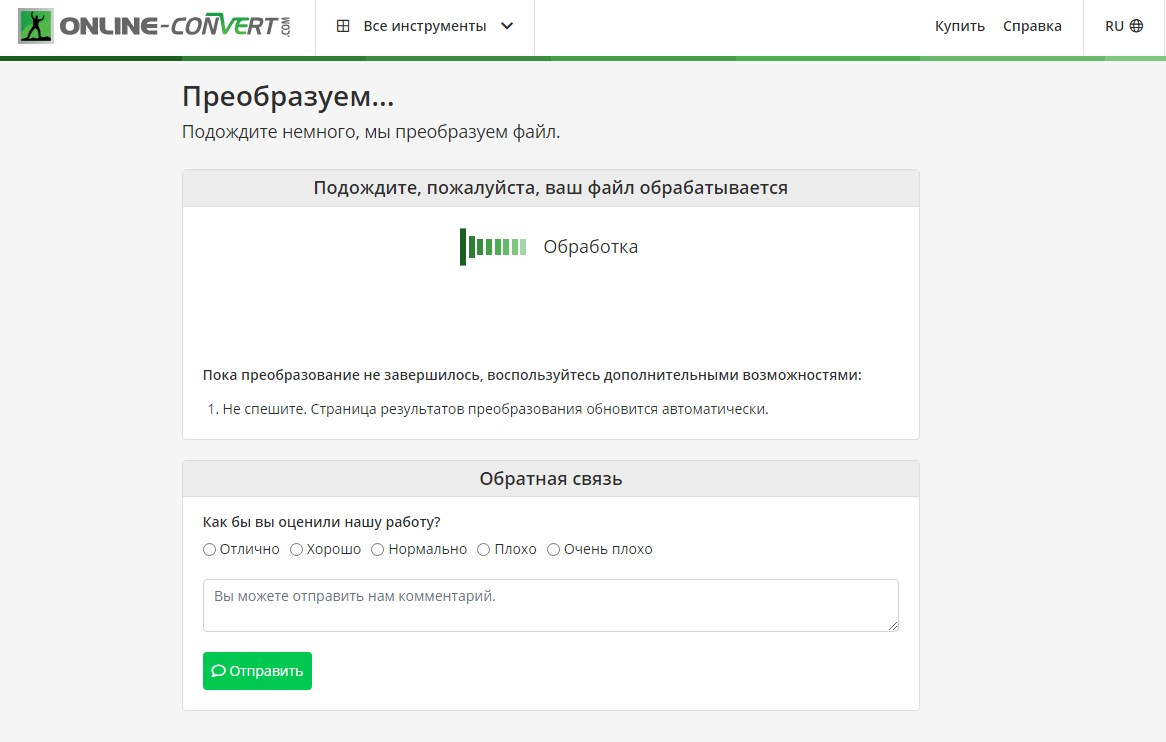
\includegraphics[width=0.8\textwidth]{img/cxp4.jpg}
\end{center}

Если вы уже обработали несколько файлов и вам скучно ждать, можно поставить оценку сервису или написать коротенький отзыв. Заметьте, сервис предоставляет такую возможность как бы «между делом», не забирая у пользователя его драгоценное время, когда он уже закончит работу с файлами, и не докучая потом сообщениями в духе «Оставьте отзыв».

\textbf{Пользовательский контроль и свобода}

Вероятность что-то не то нажать, не то загрузить или не то конвертировать есть всегда. У пользователя на каждом этапе должна быть возможность отменить действие либо удалить ошибочно загруженный или уже обработанный файл. В нашем примере сервис дает такую возможность с самого начала, как только пользователь загрузил свой файл на сайт, обозначив действие всем понятным значком в виде крестика и надписью «Удалить»:

\begin{center}
    
\includegraphics[width=0.8\textwidth]{img/cxp5.jpg}
\end{center}

Аналогичным образом можно поступить, если пользователь «спохватился» уже после того, как «отконвертил» файл. Помимо кнопок «Скачать» и «Загрузить в облако» есть кнопка «Удалить»:

\begin{center}
    
\includegraphics[width=0.8\textwidth]{img/cxp6.jpg}
\end{center}

Заметьте, что, если кнопки скачивания и загрузки выделены яркими броскими цветами, кнопка «Удалить» бледно-серая, дабы рука не тянулась к ней просто так, и пользователь не удалил готовый файл по ошибке.


\textbf{Предотвращение ошибок}

В продолжение темы следует сказать о предотвращении ошибок. Разумеется, никто не может застраховать пользователя от случайного нажатия кнопки и загрузки «не того» файла, однако обязанность разработчиков системы защитить пользователя от утечки данных и дать возможность в любой момент удалить данные не для широкого круга.

Если речь идет о более серьезных сервисах, связанных с денежными операциями, вариантом защиты может быть требование подтвердить ту или иную операцию (перевода денег, конвертации валюты и т.д.) Тут важно расставить приоритеты: сначала исключить серьезные ошибки, а затем минимизировать вероятность мелких неточностей.

Так, в нашем примере пользователь может не понять, что значить «Добавить пробный файл» и нажать эту кнопку из любопытства. Собственно, ничего страшного не происходит, и пользователь, убедившись, что это просто файл для демонстрации, как работает конвертер, может его сразу же удалить, не задерживаясь долго на странице и не отвлекаясь от своей основной задачи:

\begin{center}
    
\includegraphics[width=0.8\textwidth]{img/cxp7.jpg}
\end{center}

Такие продуманные варианты предотвращения и исправления ошибок помогают «не выпадать» из стандартной последовательности действий.

\textbf{Последовательность и стандарты}

Любой продвинутый пользователь, вынужденно или добровольно проводящий онлайн по несколько часов в день, накапливает определенный опыт взаимодействия с цифровыми продуктами, а заодно и определенный массив ожиданий, как это взаимодействие должно происходить. Мы уже поговорили про соответствие ожиданиям пользователя с самого начала взаимодействия, но этого мало.

Соответствие стандартам и традиционной последовательности операций должна наблюдаться на всех этапах взаимодействия. Интерфейс может (и должен!) подсказывать возможные действия на шаг вперед, но ни в коем случае не опережать их и не сбивать с толку. В нашем случае вполне логично, что кнопка «Начать» появляется одновременно с кнопками загрузки файла. Так пользователю не нужно гадать, что будет дальше, когда он загрузит свой файл.

Аналогичным образом весь список возможных действий должен быть представлен по окончании каждого этапа. Например, после конвертации файла помимо кнопок «Скачать», «Загрузить» и «Удалить» появляется кнопка «Преобразовать следующий файл», чтобы пользователь не раздумывал, что ему делать дальше, если ему нужно конвертировать несколько файлов:


\begin{center}
    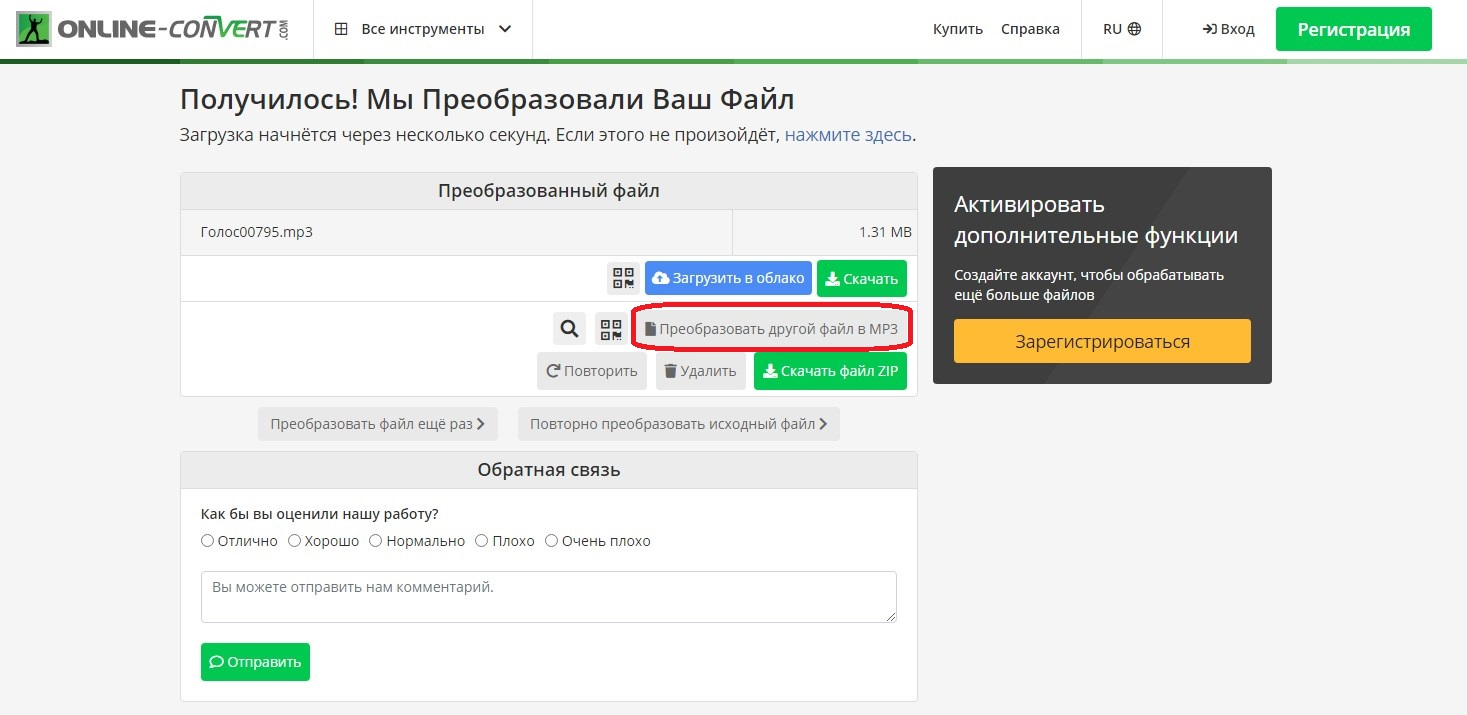
\includegraphics[width=0.8\textwidth]{img/cxp8.jpg}
\end{center}

Якоб Нильсен в своей статье отмечает, что неспособность сервиса поддерживать ожидаемую последовательность действий увеличивает когнитивную нагрузку на пользователей, когда это совершенно ни к чему [J. Nielsen, 2020]. Это примерно как стойка регистрации в отеле, что всегда расположена в холле. Если ее пришлось бы искать где-то через два коридора на другом этаже, это бы изрядно «напрягало» постояльцев отеля.

\textbf{Узнаваемость и напоминание}

Этот пункт «пересекается» с предыдущим. Чем более знакомым покажется пользователю интерфейс сайта, тем быстрее он на нем «освоится» и с тем большей вероятностью начнет заходить на этот сайт чаще. Особенно, если основной функционал сайта оправдает его ожидания.

Но данный пункт не только об этом. Он еще и том, чтобы снизить когнитивную нагрузку на пользователя даже в мелочах. Гипотетически юзер, конечно, должен помнить, какой именно файл он загрузил для конвертации минуту тому назад. Однако человека могут отвлечь какие-то дела, мысли, звонки. А если файлов много, можно просто сбиться со счета, потому как бесплатный сегмент сервиса позволяет конвертировать не более одного файла за один заход.

Именно поэтому основная информация об операции должна дублироваться на каждой странице каждого последующего шага. В нашем случае пользователь видит название загруженного файла как собственно при загрузке, так и после обработки:

\begin{center}
    
\includegraphics[width=0.8\textwidth]{img/cxp9.jpg}
\end{center}

К слову, это относится не только к оперативной информации, которая должна быть «на виду» и «под рукой». Аналогичным образом следует выстроить справочное сопровождение и помощь, предлагая ее в контексте возникшей проблемы, а не сразу весь мануал, 95\% из которого пользователю никогда не понадобится.


\textbf{Справочная информация}

Тем не менее, у пользователя должна быть возможность в любой момент найти ответ на любой свой вопрос, пусть даже пока у него никаких проблем не возникло. Раздел «Справка» должен быть на видном месте, лучше в верхнем меню, и структурирован на основные темы запросов пользователей:

\begin{center}
    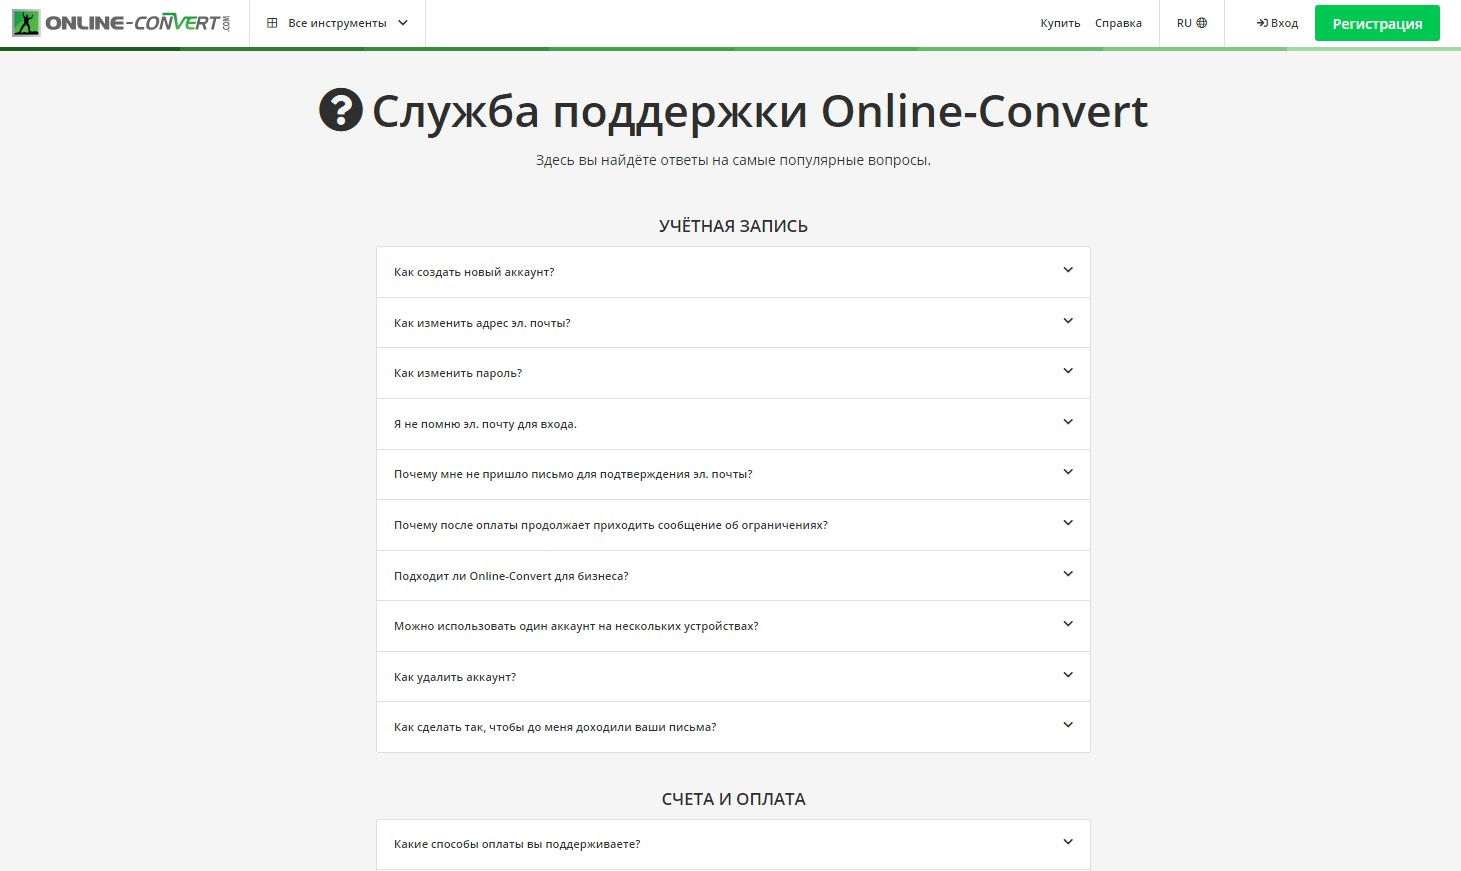
\includegraphics[width=0.8\textwidth]{img/cxp10.jpg}
\end{center}

Это, кстати, существенно разгрузит службу технической поддержки, потому что основной массив вопросов составляют одни и те же часто повторяющиеся проблемы, зачастую не имеющие никакого отношения собственно к сервису, а обусловленные человеческим фактором (забыл, не помню, не понял и т.д.). Разумеется, такого рода вопросы тоже должны быть обеспечены ответами.

\textbf{Гибкость использования}

Про индивидуальный подход слышали все, но не все разработчики вняли. Так, гибкость процессов – это «наше все». Не нужно «грузить» человека, которому нужно конвертировать один файл, информацией о годовой подписке. Эту информацию нужно предоставить только зарегистрированным пользователям.

Следует внятно написать, что именно даст регистрация на сайте и зачем она в принципе нужна. Например, для того, чтобы за один заход обрабатывать больше файлов, а не один, как в бесплатной версии:

\begin{center}
    
\includegraphics[width=0.8\textwidth]{img/cxp11.jpg}
\end{center}

Такая прозрачность избавит пользователя от возможных разочарований, а владельцев сайта – от негативных отзывов недовольных посетителей, потративших время на регистрацию непонятно зачем.

\textbf{Минимализм в дизайне}

Данный пункт связан со всеми предыдущими пунктами сразу. Если держать в фокусе только актуальную необходимую информацию, текущее действие и следующие возможные шаги, нет никакой необходимости перегружать сайт лишней информацией, картинками, элементами дизайна. Вот и не перегружайте.

Выражаясь научным языком, каждая дополнительная единица информации в интерфейсе конкурирует с другими единицами информации, в результате чего снижается относительная видимость каждой единицы информации [J. Nielsen, 2020].


\textbf{Помощь пользователям}

Про помощь пользователям в обращении с интерфейсом и использовании сервиса мы поговорили достаточно подробно. Однако могут возникнуть не зависящие от владельца сайта обстоятельства, мешающие воспользоваться сервисом. Например, прервется онлайн-соединение.

Сообщить об этом нужно простым и понятным языком: «Проверьте подключение к Интернету». Лучше не писать «Нет Интернета», потому что так пользователю может быть не совсем понятно, у кого именно нет интернет-соединения: у него или у вас.

Это и есть 10 эвристик юзабилити для дизайна пользовательского интерфейса. К слову, первоначальный вариант статьи Якоб Нильсен написал в далеком 1994 году, а в 2020 году только дополнил и расширил статью с учетом актуальной информации. Тем не менее, все базовые постулаты остались прежними. Как метко заметил автор, если что-то работает и остается неизменным на протяжении почти 30 лет, весьма вероятно, что это будет актуально еще достаточно долго.

Так что все эти рекомендации лучше соблюдать. В противном случае можно наделать много досадных ошибок, которые будут снижать конверсию и отпугивать пользователей.

\textbf{Основные ошибки в дизайне по Нильсену}

Какие ошибки можно совершить, проектируя дизайн интерфейса? Подробно об этом рассказал сам Якоб Нильсен в своей работе Top 10 Mistakes in Web Design («Топ-10 ошибок в веб-дизайне») [J. Nielsen, 2011]. Тут очень много самоочевидного, но почему-то все еще не воспринимаемого дизайнерами, разработчиками и заказчиками цифровых продуктов. Поэтому ограничимся просто списком с короткими пояснениями.

Топ-10 ошибок в веб-дизайне:

\begin{enumerate}
    \item Неудобный поиск – когда невозможно ничего найти, когда результат поиска нерелевантен запросу, когда на короткий внятный вопрос «выпадает» мануал на 150 страниц и т.д.
    \item PDF-файлы для онлайн-чтения – они оптимизированы под формат А4, а не под размер экрана, из-за чего возникает множество неудобств, начиная от мелкого шрифта и заканчивая неудобной прокруткой.
    \item Ранее просмотренные пользователем ссылки не меняют цвет – в итоге легко запутаться, особенно, если на сайте много контента.
    \item Нечитаемый текст – отсутствие разбивки на абзацы, слишком длинные абзацы, отсутствие разделов, подразделов и какой-то внятной структуры, избыток узкоспециальных терминов и профессионального жаргона.
    \item Фиксированный размер шрифта – не подходит для людей с не очень хорошим зрением, не желающим носить очки.
    \item Сходство с рекламой – если какой-либо раздел сайта похож на рекламу, его с высокой долей вероятности просто не станут изучать.
    \item Появление новых окон в браузере – это примерно как с рекламой, поэтому даже очень нужное окно чата с ботом лучше предлагать не сразу, а хотя бы через полминуты, чтобы пользователь успел «осмотреться» на сайте.
    \item Вопросы без ответов – когда ответ нельзя найти ни через поиск, ни через бот, ни через раздел «Справка», ни собственно в разделе сайта. Либо когда отсутствует информация, которая должна наличествовать по умолчанию. Например, цена товара в интернет-магазине.
    \item Нарушение общепринятых правил дизайна – меню должно быть вверху, строка поиска тоже вверху, кнопка «В корзину» вверху справа и т.д. Если такие общепонятные вещи приходится искать непонятно где, пользователь чаще всего просто уходит с сайта.
    \item Заголовки страниц не оптимизированы под поисковые системы – есть риск, что в этом случае даже очень ценная информация так и не попадет к пользователю. «Добро пожаловать» и «Внимание» не подходят, равно как и «Интересное предложение», «Акция», «Скидка» без пояснений, к чему это все относится.
\end{enumerate}

Небольшая подсказка к последнему пункту: заголовок страницы содержится внутри HTML-тега и почти всегда используется в качестве кликабельного заголовка среди результатов выдачи поисковых систем (SERP). Это для тех, кто хочет заняться оптимизацией сайта лично.

Итак, мы достаточно подробно рассмотрели все нюансы закона Якоба Нильсена. Осталось только им безоговорочно следовать… Или нет?.. Некоторые считают, что нет.


\textbf{Нюансы интерпретации закона Якоба Нильсена}

Сразу скажем, откуда взялся скептицизм в отношении закона Якоба Нильсена. И, кстати, не только в отношении него. Есть такая интересная статья «Ошибки в интерпретации UX законов: неверно понятые правила UX» [Р. Наджафов, 2022]. Тут, правда, больше не об ошибках, а о том, что все хорошо в меру.

Закон Якоба Нильсена частенько интерпретируют как призыв к примитивизму, отказу от эксперимента и креатива, использованию готовых шаблонов на все случаи жизни, потому что пользователям нужен узнаваемый дизайн, интуитивно понятный функционал и т.д. Имел ли это в виду сам Якоб Нильсен?

Вряд ли, потому что удобная навигация по сайту и креативные картинки к статьям в блоге никоим образом не исключают друг друга. Кроме того, вполне можно как-то нешаблонно сказать пользователю «Спасибо» за то, что он воспользовался вашим сервисом, когда он уже получит желаемый результат и точно не отвлечется от процесса на картинку с котиком, вручающим ему букет цветов.

Кроме того, новые впечатления поднимают настроение, а за хорошим настроением пользователь всегда охотно вернется на понравившийся сайт. Поэтому повторимся, что все хорошо в меру, во всем нужен баланс, а шаблоны и стандарты нужны исключительно для обеспечения удобства пользования.
